\documentclass[11pt, a4paper]{article}

% --- Packages ---
\usepackage[utf8]{inputenc}
\usepackage[T1]{fontenc}
\usepackage{geometry}
\geometry{a4paper, margin=1in}
\usepackage{amsmath, amssymb, amsthm}
\usepackage{graphicx}
\usepackage{hyperref}
\usepackage{xcolor}
\usepackage{enumitem}
\usepackage{booktabs}
\usepackage{longtable}
\usepackage{multirow}
\usepackage{array}

% --- Bibliography Setup ---
\usepackage[backend=biber, style=numeric, sorting=nyt]{biblatex}
\addbibresource{references.bib}

% --- Metadata ---
\title{Strategic Analysis of Card-Based Liar's Poker:\\
       Combinatorial Foundations and Nash Equilibrium Approximation}
\author{Connor M. Lockhart \\ \texttt{connorl@umd.edu} \\ \textit{University of Maryland}}
\date{\today}

% --- Environments ---
\newtheorem{theorem}{Theorem}
\newtheorem{lemma}[theorem]{Lemma}
\theoremstyle{definition}
\newtheorem{definition}{Definition}
\newtheorem{example}{Example}
\newtheorem{remark}{Remark}

\begin{document}

\maketitle

\begin{abstract}
We study a card-based variant of Liar's Poker played with a standard 52-card deck, where
players bid on the quality of the combined pool of all players' hidden hands using standard
poker hand rankings. The game proceeds through a series of escalating bids until a player
calls ``bullshit,'' triggering a pool-wide reveal. A player is eliminated upon accumulating
five cards. This paper establishes the combinatorial foundations for rational play by
computing exact hand-type probabilities for pool sizes $n = 5$ through $n = 25$ cards,
enabling provably optimal ``blind'' bidding strategies that require no private information.
We further characterize how a player's private hand shifts the probability distribution
over pool outcomes, quantifying the information value of observing one's own cards. These
results provide the analytical groundwork for a forthcoming implementation of a
Regularized Nash Dynamics (RND) agent~\cite{rnd_paper} trained via self-play, using the
OpenSpiel framework~\cite{openspiel} as a computational backbone.
\end{abstract}

\section{Introduction}

Liar's Poker occupies a unique position in the landscape of imperfect-information games:
it combines probabilistic reasoning over a shared hidden state with strategic bluffing and
adversarial inference. The card-based variant studied here departs from the
dollar-bill version popularized in finance by instead using poker hand rankings to define
the bid space, creating a richer and more complex strategic environment.

%The game is of theoretical interest for several reasons. ADD THESE 

This paper makes the following contributions:
\begin{enumerate}
    \item We provide exact combinatorial probabilities for all ten standard poker hand
          types for pool sizes $n = 5$ to $n = 25$ cards drawn from a 52-card deck
          (Section~\ref{sec:blind}), establishing a principled basis for blind bidding
          strategy.
    \item We quantify the conditional shift in pool-hand probabilities given a player's
          private hand (Section~\ref{sec:conditional}), characterizing the value of
          private information.
    \item We outline the game-theoretic framework and plan for a Regularized Nash
          Dynamics agent~\cite{rnd_paper} to approximate the Nash equilibrium of the game
          (Section~\ref{sec:future}).
\end{enumerate}

\section{Game Rules and Formal Model}
\label{sec:rules}

\subsection{Setup and Play}

The game is played by $k \in \{2, 3, 4, 5\}$ players using a standard 52-card deck.
At the start of each round, every player is dealt exactly one card face-down from a
freshly shuffled deck. Players may look at their own card at any time but may never
reveal it to other players.

\begin{definition}[Hand Pool]
The \emph{hand pool} is the multiset of all cards currently held by all active players.
If player $i$ holds $h_i$ cards, the pool has size $n = \sum_i h_i$.
\end{definition}

\begin{definition}[Pool Hand]
The \emph{pool hand} is the best standard 5-card poker hand achievable from any five
cards selected from the hand pool. Hand types, from lowest to highest, are:
\[
\text{High Card} < \text{Pair} < \text{Two Pair} < \text{Three of a Kind} < \text{Straight}<\]
\[ \text{Flush} < \text{Full House} < \text{Four of a Kind} < \text{Straight Flush} < \text{Royal Flush.}
\]
\end{definition}

\subsection{Bidding Protocol}

Play proceeds in turns in a fixed circular order. On each turn, the active player must
choose one of two actions:

\begin{enumerate}
    \item \textbf{Bid:} Name a poker hand $(T, r)$ where $T$ is a hand type and $r$ is
          a primary rank specifier. The bid asserts that the hand pool contains a
          5-card combination of type $T$ at rank $r$ or better. The bid must be
          strictly higher than the previous bid, where bids are ordered first by hand
          type $T$, then by primary rank $r$ within the same type.
    \item \textbf{Call:} Challenge the previous bidder's claim.
          All cards in the hand pool are then revealed and the pool hand is evaluated.
\end{enumerate}

\begin{definition}[Bid Ordering]
Bid $(T_1, r_1) > (T_2, r_2)$ if and only if $T_1 > T_2$, or $T_1 = T_2$ and
$r_1 > r_2$. The first bid of a round may be any valid bid.
\end{definition}

\subsection{Challenge Resolution and Elimination}

When a player calls, the hand pool is revealed and the pool hand is evaluated.

\begin{itemize}
    \item \textbf{Correct call} (the claimed hand does \emph{not} exist in the pool):
          The player who made the false bid receives one additional card dealt from
          the deck.
    \item \textbf{Incorrect call} (the claimed hand \emph{does} exist in the pool):
          The player who called receives one additional card dealt from the deck.
\end{itemize}

In both cases, the player who gains a card now holds one more card for subsequent rounds.

\begin{definition}[Elimination]
A player is \emph{eliminated} when they hold 5 or more cards. The last remaining
player wins the game.
\end{definition}

\begin{remark}
The symmetric penalty structure---both incorrect bids and incorrect challenges result
in receiving an additional card---creates an asymmetric strategic landscape. Because
cards accumulate toward the elimination threshold, \emph{both} bluffing too aggressively
(risking a correct challenge) and challenging too aggressively (risking an incorrect
call) are penalized. This balance is central to the Nash equilibrium analysis.
\end{remark}

\begin{example}[Two-Player Round]
Players $A$ and $B$ each hold 2 cards. The pool has size $n=4$. Player $A$ bids
``Pair of Kings.'' Player $B$ calls. The four cards are revealed; suppose the pool
contains $\{\clubsuit A, \heartsuit A, \diamondsuit 7, \spadesuit 3\}$. The pool hand
is ``Pair of Aces,'' so the bid was valid. $B$'s call was incorrect: $B$ receives a
card and now holds 3 cards for the next round.
\end{example}

\section{Combinatorial Probability Analysis}
\label{sec:prob}

\subsection{Blind Strategy: Marginal Hand Probabilities}
\label{sec:blind}

A \emph{blind strategy} is one that ignores the player's own cards and reasons solely
from the pool size $n$. While not optimal in general, blind strategies provide
principled lower bounds on rational bidding: if a hand type has probability $p < 0.5$
of appearing in a pool of size $n$, then bidding that type is disadvantageous without
additional private information supporting the claim.

\begin{definition}[Marginal Hand Probability]
For a pool of $n$ cards drawn uniformly at random (without replacement) from a
52-card deck, the marginal probability of hand type $T$ is
\[
P(T, n) = \frac{|\{\,S \subseteq \binom{[52]}{n} : \text{best hand of } S = T\,\}|}{\binom{52}{n}}.
\]
\end{definition}

Figure~\ref{fig:blind_probs} shows $P(T, n)$ for all ten hand types and pool sizes
$n = 5$ through $n = 25$. For $n \in \{5, 6, 7\}$, values are exact combinatorial
counts from published enumeration. For $n \geq 8$, values are computed via Monte Carlo
simulation with $N = 3 \times 10^6$ samples per pool size; standard errors are below
$0.01\%$ for all reported values.

Wu and Wu~\cite{wu2024ncard} derive closed-form combinatorial formulas for the counts
of $n$-card hands \emph{containing} a straight, flush, or full house pattern for
arbitrary $n$. Their exact counts serve as external validation of our Monte Carlo
estimates and reveal two crossover points in the probability ordering of these hands:
flush surpasses straight in occurrence frequency at $n = 12$, and full house surpasses
straight at $n = 20$ (in the sense that more hands \emph{contain} these patterns at
those pool sizes).
Note that Wu and Wu's definition counts any hand that contains the relevant pattern---including
hands where a strictly better 5-card combination is also available---whereas our $P(T,n)$
records only the \emph{best} achievable hand type. The two definitions coincide for
$n \leq 7$ and diverge gradually for larger $n$ as multi-pattern hands become common.

\begin{figure}[h!]
    \centering
    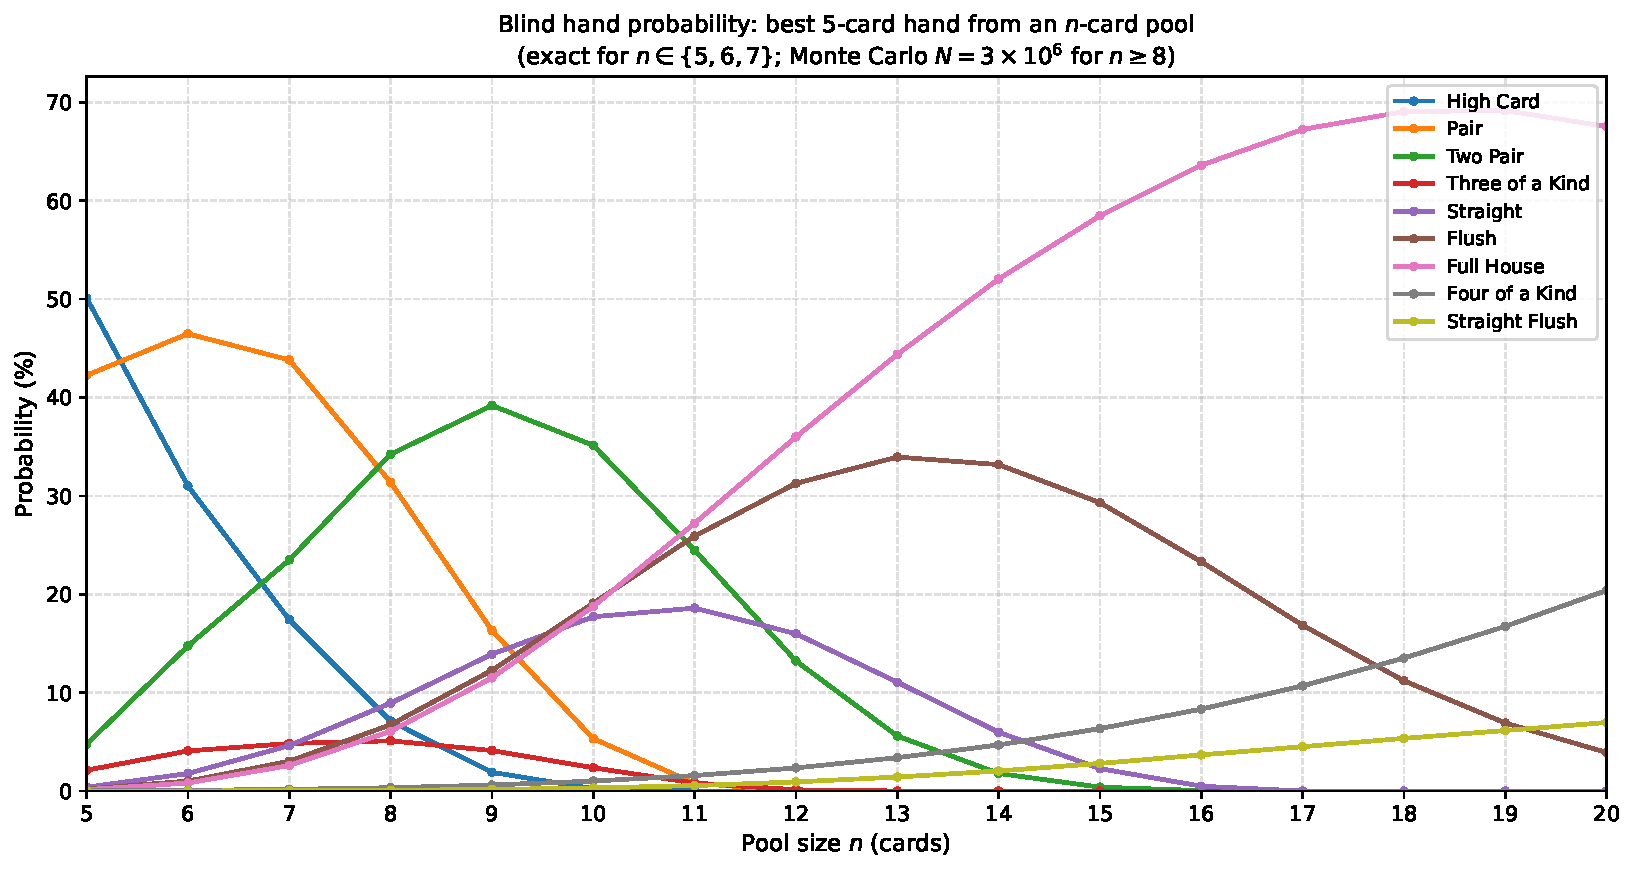
\includegraphics[width=\textwidth]{figures/hand_probabilities.pdf}
    \caption{Probability of each best hand type as a function of pool size $n$
             (Royal Flush omitted; probability $< 3\%$ across the entire range).
             Generated by \texttt{generate\_prob\_tables.py}.}
    \label{fig:blind_probs}
\end{figure}

\begin{figure}[h!]
    \centering
    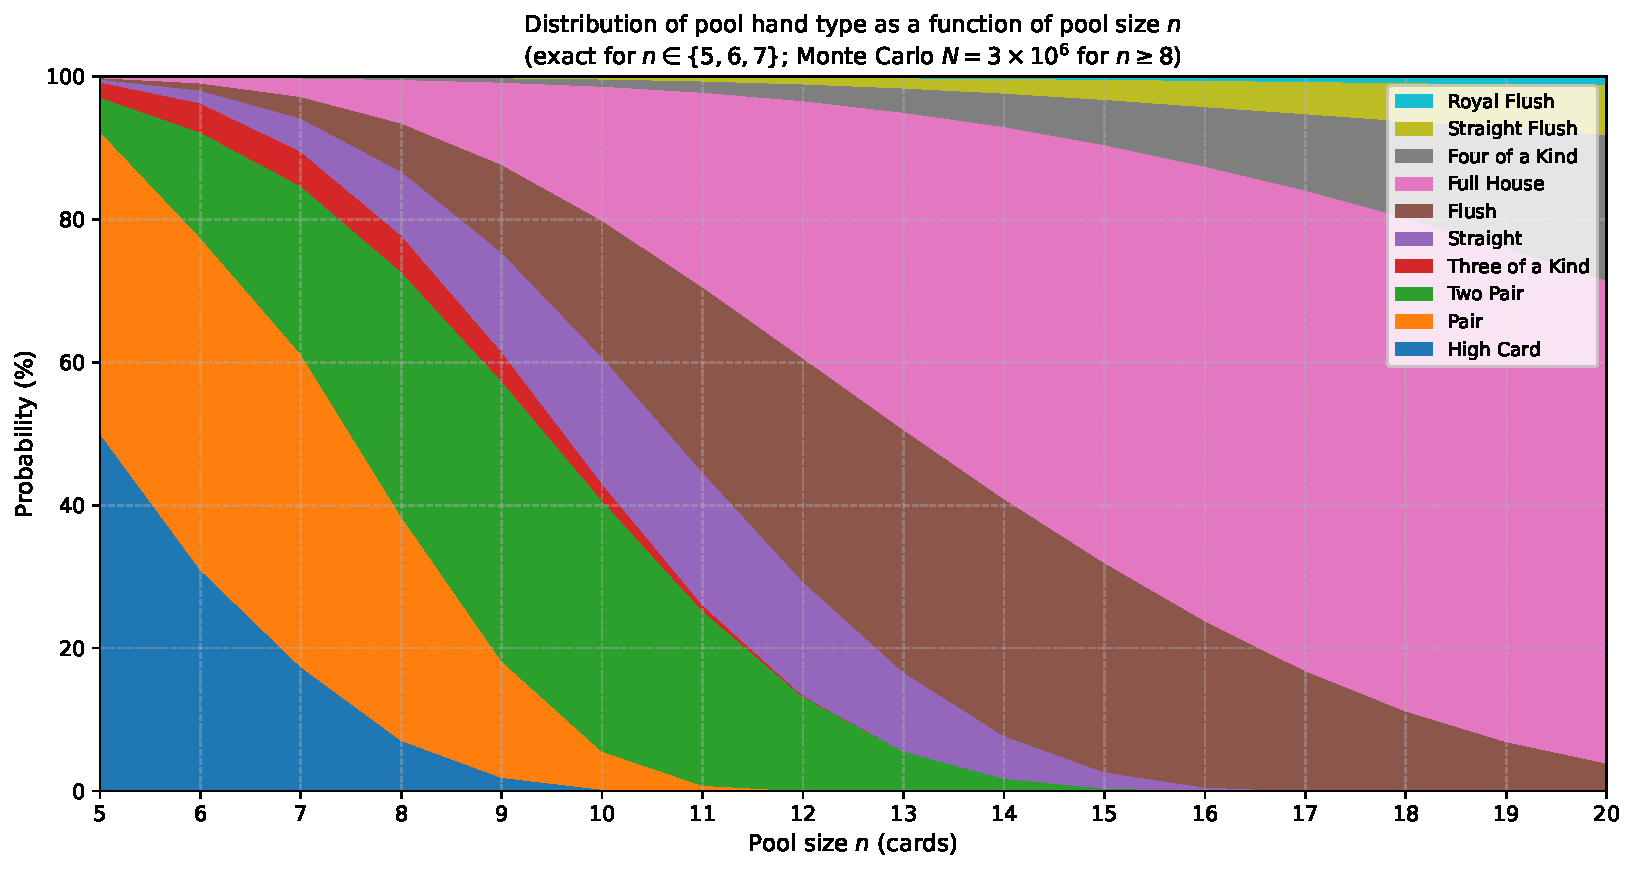
\includegraphics[width=\textwidth]{figures/hand_distribution.pdf}
    \caption{Stacked area chart showing how the full distribution of pool hand types
             shifts with pool size $n$. Each band gives $P(T, n)$; bands sum to 100\%.
             Generated by \texttt{generate\_prob\_tables.py}.}
    \label{fig:hand_distribution}
\end{figure}

\begin{figure}[h!]
    \centering
    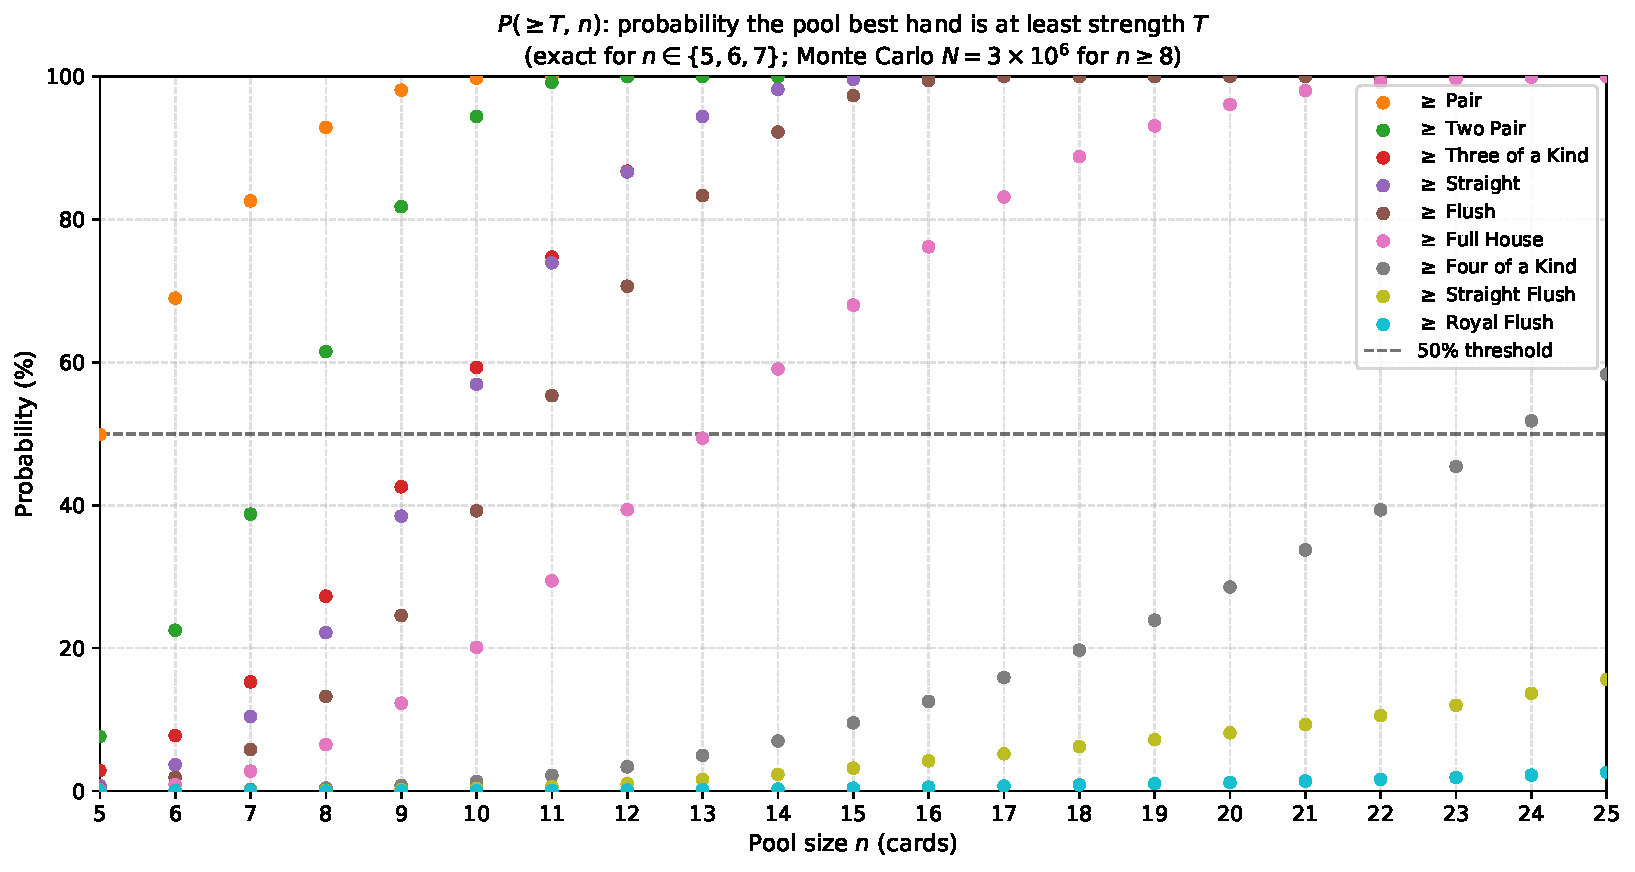
\includegraphics[width=\textwidth]{figures/hand_at_least.pdf}
    \caption{Cumulative ``at-least'' probability $P(\geq T, n) = \sum_{T' \geq T} P(T', n)$
             for each hand type $T$ as a function of pool size $n$.
             A value of 50\% marks the threshold above which a blind bid on hand type $T$
             is better than chance.
             Generated by \texttt{generate\_prob\_tables.py}.}
    \label{fig:at_least}
\end{figure}

\subsection{Conditional Probabilities Given Private Information}
\label{sec:conditional}

In practice, each player knows their own cards. This section quantifies how private
hand knowledge shifts the probability distribution over pool hand types.

\begin{definition}[Conditional Pool Probability]
Let $\mathbf{h}$ be the set of cards held by player $i$, achieving private hand type
$X = \mathrm{BestHand}(\mathbf{h})$. For a pool of total size $n$ (including
$|\mathbf{h}|$ of the player's own cards and $n - |\mathbf{h}|$ opponent cards drawn
from the remaining $52 - |\mathbf{h}|$ cards), the conditional pool probability is
\[
P(T \mid X, n) = \Pr[\mathrm{BestHand}(\mathbf{h} \cup \mathbf{o}) = T],
\]
where $\mathbf{o}$ is drawn uniformly from $\binom{[52] \setminus \mathbf{h}}{n - |\mathbf{h}|}$.
\end{definition}

The following subsections examine $P(T \mid \mathbf{h}, n)$ and the corresponding
cumulative $P(\geq T \mid \mathbf{h}, n)$ for five private hand conditions.
In each figure, dashed lines reproduce the blind baseline from
Section~\ref{sec:blind} and solid lines show the conditional distribution.
All conditional figures are generated via Monte Carlo with $N = 1{,}000{,}000$
samples (\texttt{compute\_conditional\_probs.py}).

\clearpage
\subsubsection{Paired and Grouped Cards}

\begin{figure}[h!]
    \centering
    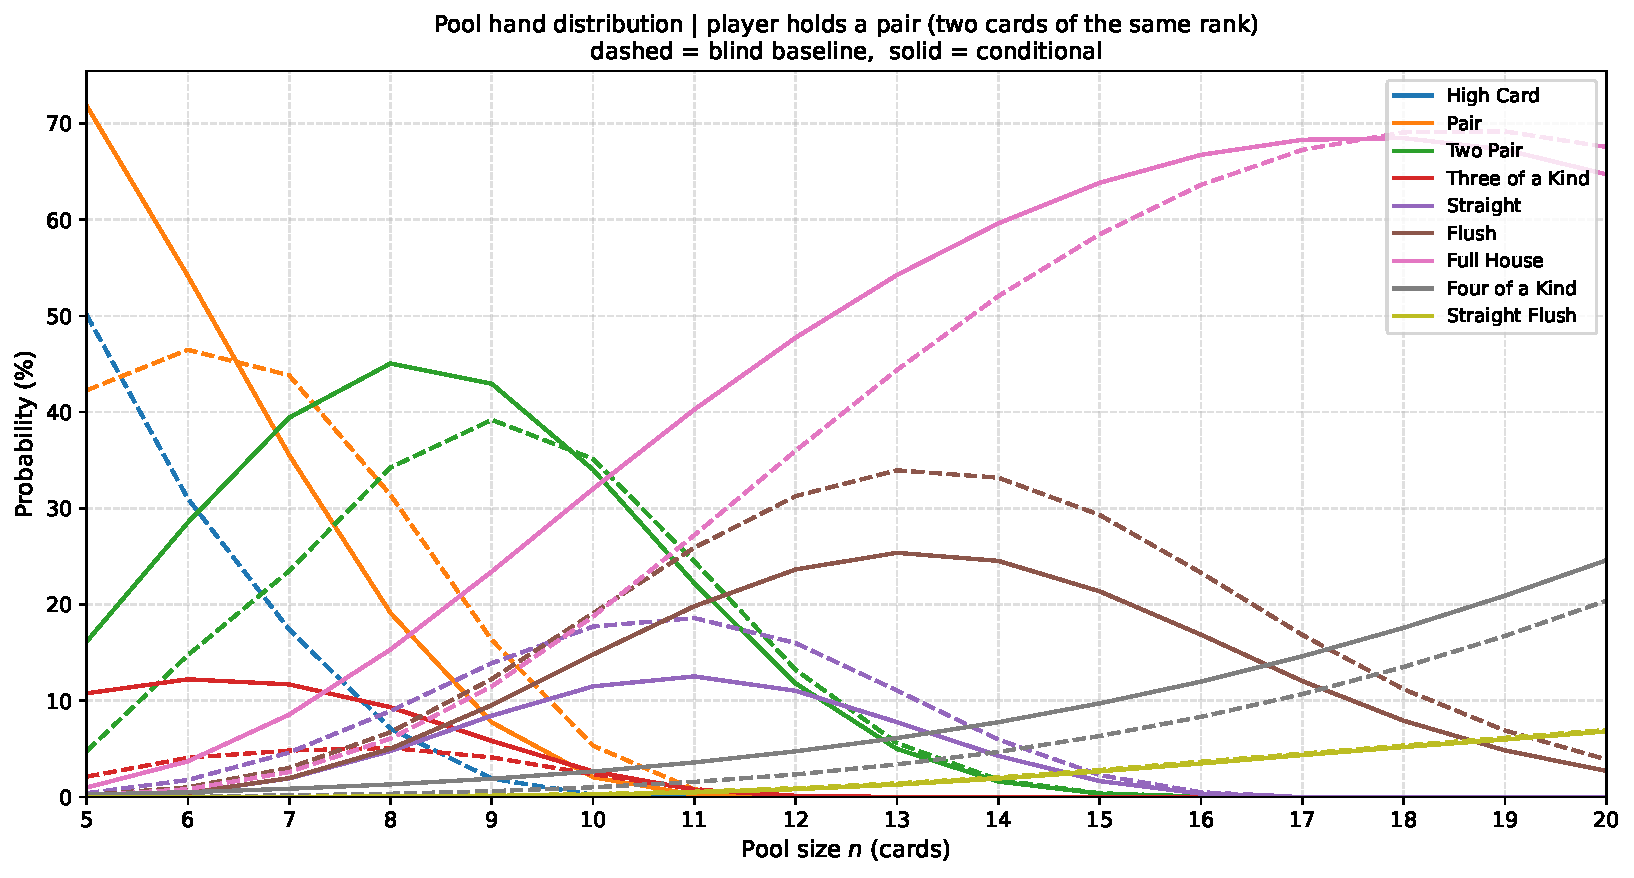
\includegraphics[width=\textwidth]{figures/conditional_pair.pdf}
    \caption{Conditional pool-hand distribution given the player holds a \emph{pair}
             (two cards of the same rank). Dashed = blind baseline; solid = conditional.}
    \label{fig:cond_pair}
\end{figure}

\begin{figure}[h!]
    \centering
    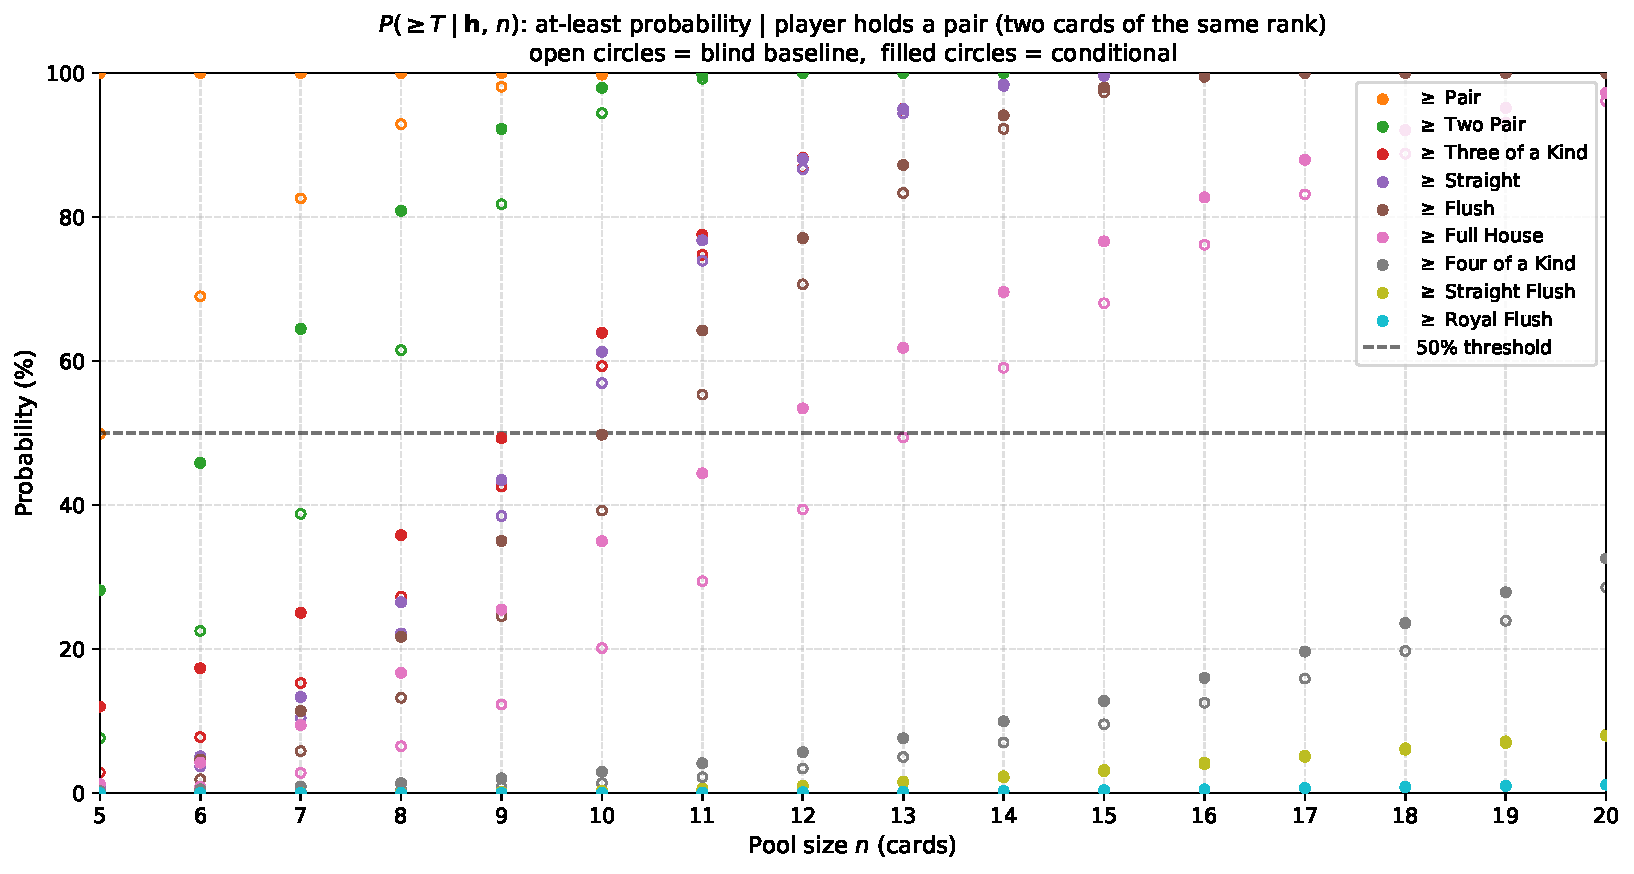
\includegraphics[width=\textwidth]{figures/conditional_pair_atleast.pdf}
    \caption{Cumulative at-least probability $P(\geq T \mid \mathbf{h}, n)$ given
             the player holds a \emph{pair}.
             Open circles = blind baseline; filled circles = conditional; dashed = 50\% threshold.}
    \label{fig:cond_pair_al}
\end{figure}

\begin{figure}[h!]
    \centering
    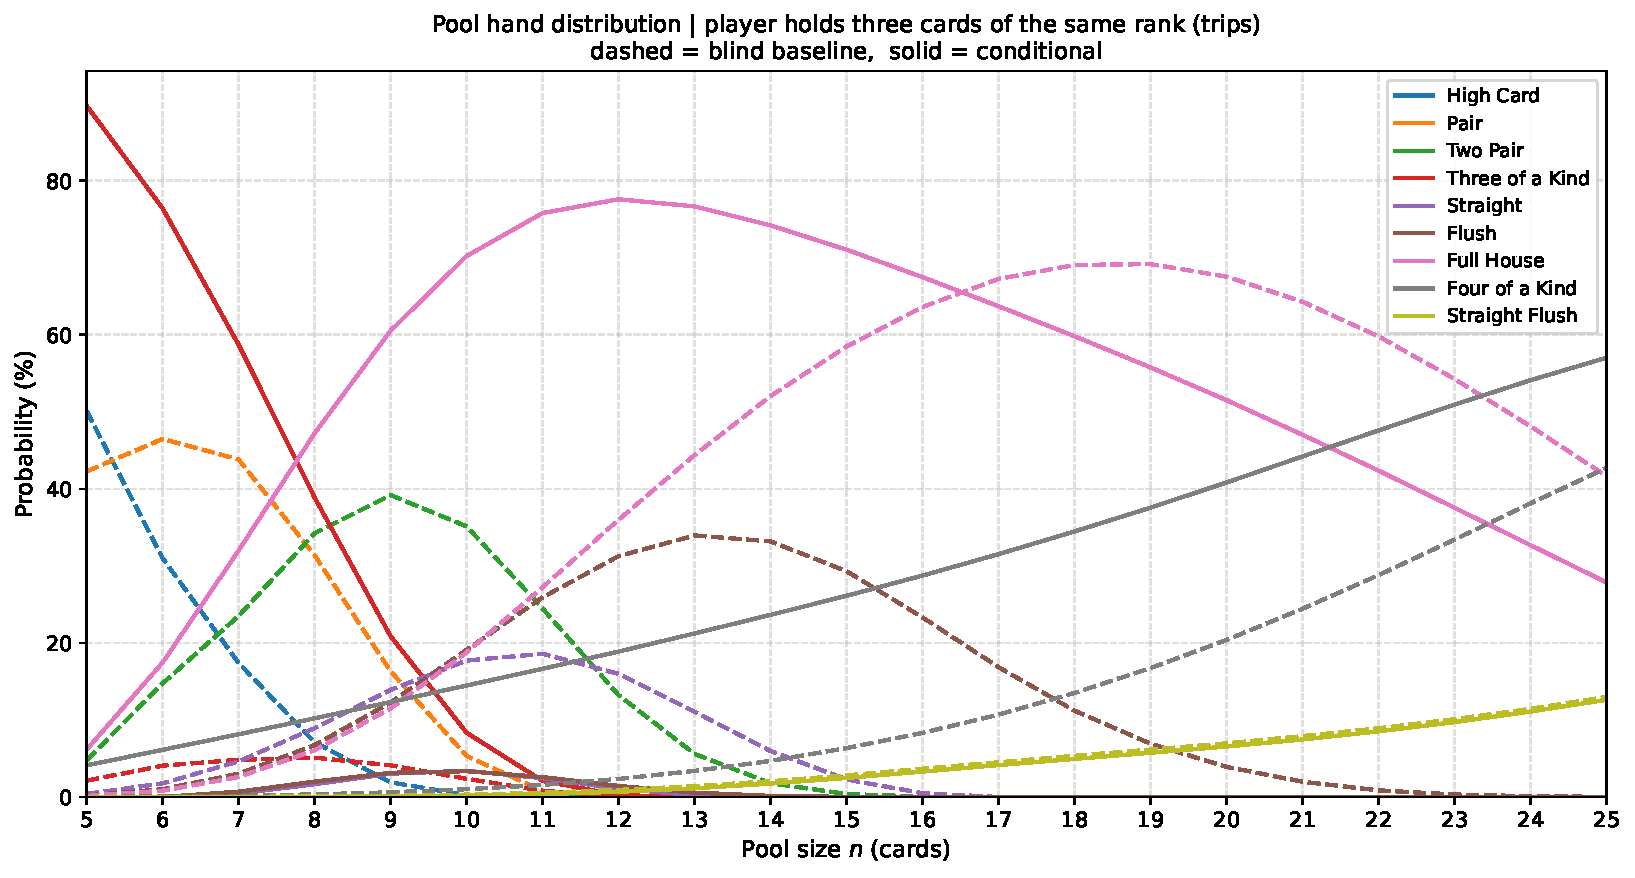
\includegraphics[width=\textwidth]{figures/conditional_trips.pdf}
    \caption{Conditional pool-hand distribution given the player holds \emph{trips}
             (three cards of the same rank). Dashed = blind baseline; solid = conditional.}
    \label{fig:cond_trips}
\end{figure}

\begin{figure}[h!]
    \centering
    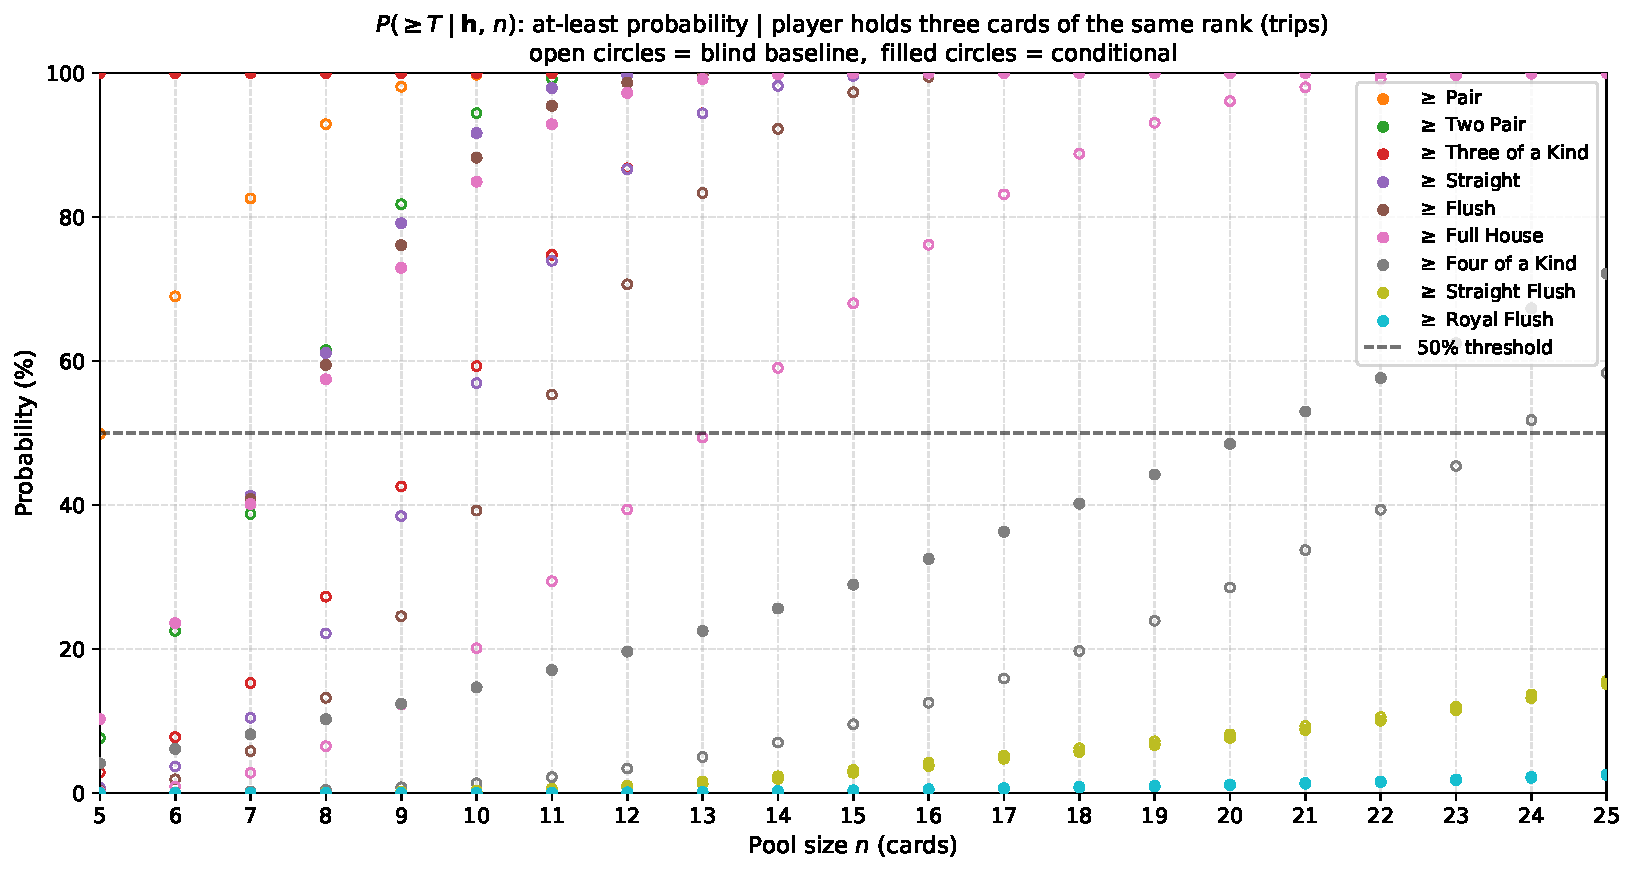
\includegraphics[width=\textwidth]{figures/conditional_trips_atleast.pdf}
    \caption{Cumulative at-least probability $P(\geq T \mid \mathbf{h}, n)$ given
             the player holds \emph{trips}.
             Open circles = blind baseline; filled circles = conditional; dashed = 50\% threshold.}
    \label{fig:cond_trips_al}
\end{figure}

Holding a pair eliminates the possibility of a High Card pool outcome entirely across all pool
sizes. At $n = 7$, the Two Pair probability rises by $+15.9$ pp to $39.4\%$, Three of a Kind
by $+6.9$ pp to $11.7\%$, and Full House by $+6.0$ pp to $8.6\%$ relative to the blind
baseline; Straight and Flush are suppressed by $2.7$ and $1.1$ pp respectively.
At $n = 10$, the Full House elevation reaches $+13.3$ pp ($32.0\%$ vs.\ $18.8\%$), while
Straight and Flush are reduced by $6.2$ and $4.3$ pp.
At $n = 14$, the Flush suppression grows to $-8.6$ pp ($24.5\%$ vs.\ $33.2\%$) and the Full
House premium narrows to $+7.6$ pp.
These shifts support elevated bids on Full House and Four of a Kind relative to blind strategy
and discount Straight and Flush bids at moderate pool sizes.

Holding trips eliminates High Card, Pair, and Two Pair as possible pool outcomes entirely.
At $n = 7$, Three of a Kind rises by $+53.9$ pp to $58.7\%$ and Full House by $+29.4$ pp to
$32.0\%$, with Four of a Kind elevated to $8.1\%$ ($+8.0$ pp).
At $n = 10$, Full House dominates at $70.2\%$ ($+51.5$ pp) and Four of a Kind rises to $14.5\%$
($+13.5$ pp); Straight and Flush are suppressed by $14.3$ and $15.7$ pp respectively.
At $n = 14$, Four of a Kind reaches $23.6\%$ ($+19.0$ pp) and Full House $74.2\%$ ($+22.2$ pp),
while Flush is nearly entirely eliminated.
At $n = 20$, Four of a Kind overtakes the relative distribution at $40.8\%$ ($+20.4$ pp),
an inversion relative to the baseline in which Full House remains the dominant outcome.

\clearpage
\subsubsection{Suited Cards}

\begin{figure}[h!]
    \centering
    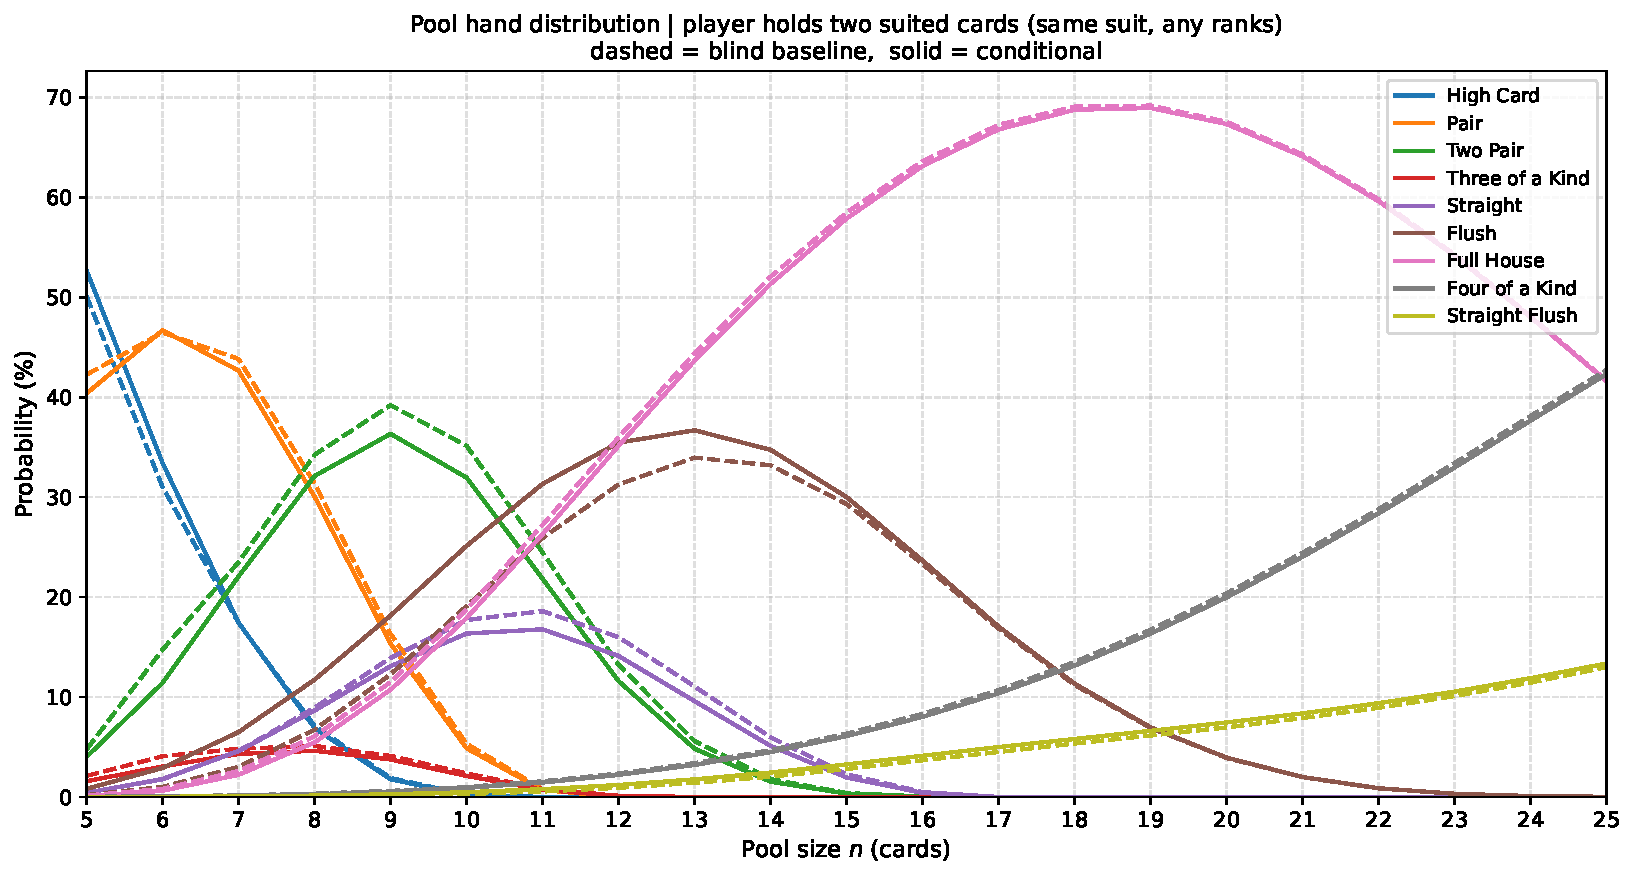
\includegraphics[width=\textwidth]{figures/conditional_suited.pdf}
    \caption{Conditional pool-hand distribution given the player holds two
             \emph{suited cards} (same suit, any ranks).
             Dashed = blind baseline; solid = conditional.}
    \label{fig:cond_suited}
\end{figure}

\begin{figure}[h!]
    \centering
    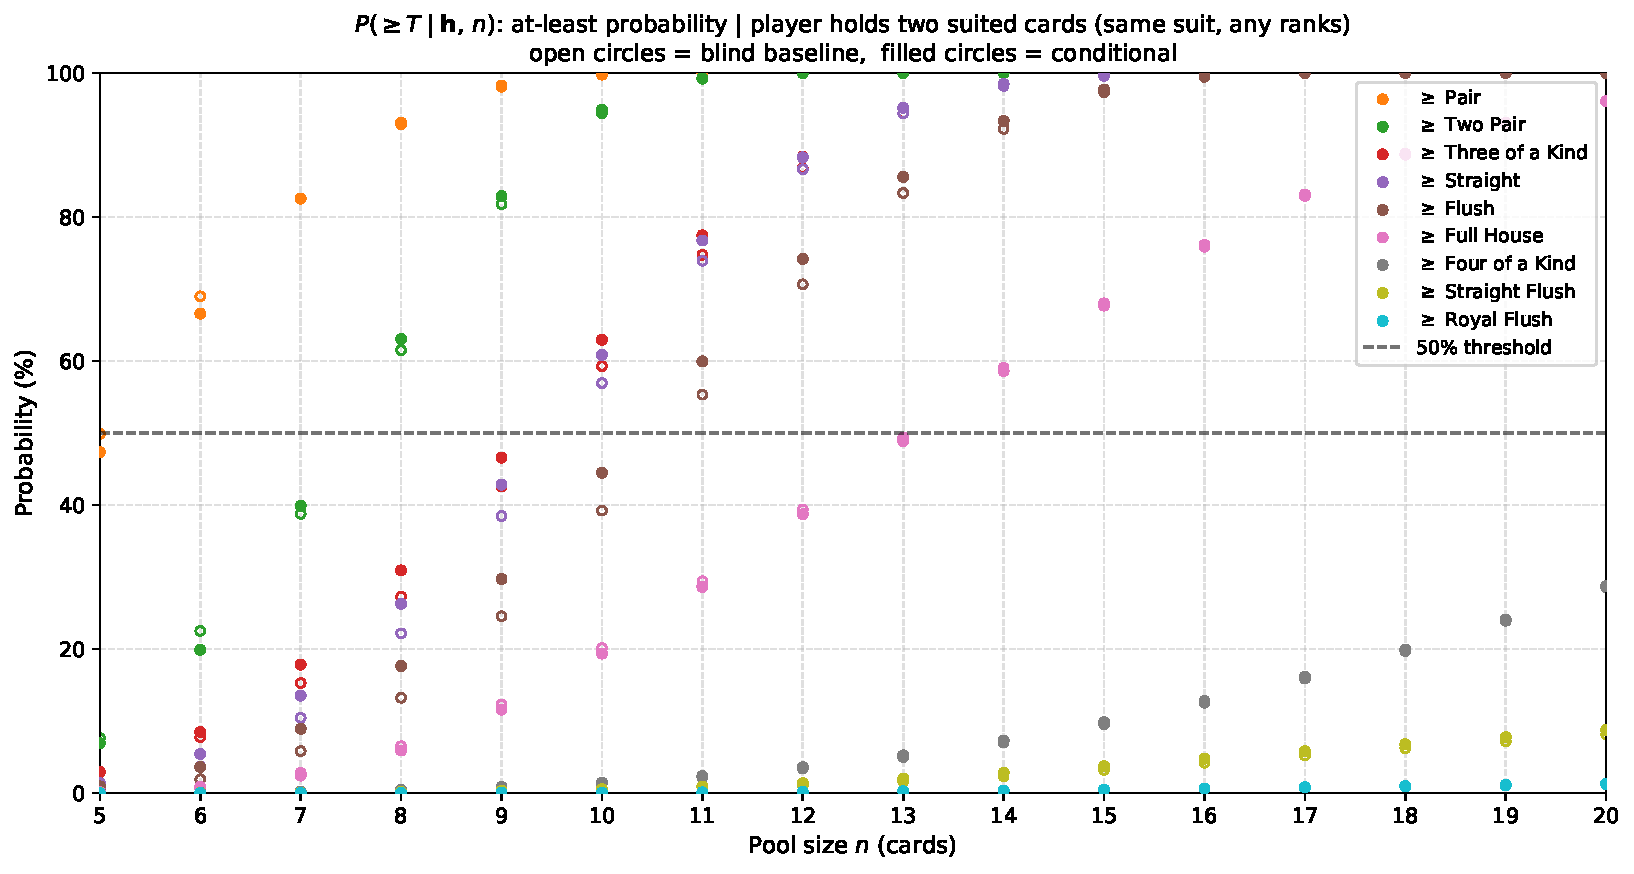
\includegraphics[width=\textwidth]{figures/conditional_suited_atleast.pdf}
    \caption{Cumulative at-least probability $P(\geq T \mid \mathbf{h}, n)$ given
             the player holds \emph{two suited cards}.
             Open circles = blind baseline; filled circles = conditional; dashed = 50\% threshold.}
    \label{fig:cond_suited_al}
\end{figure}

\begin{figure}[h!]
    \centering
    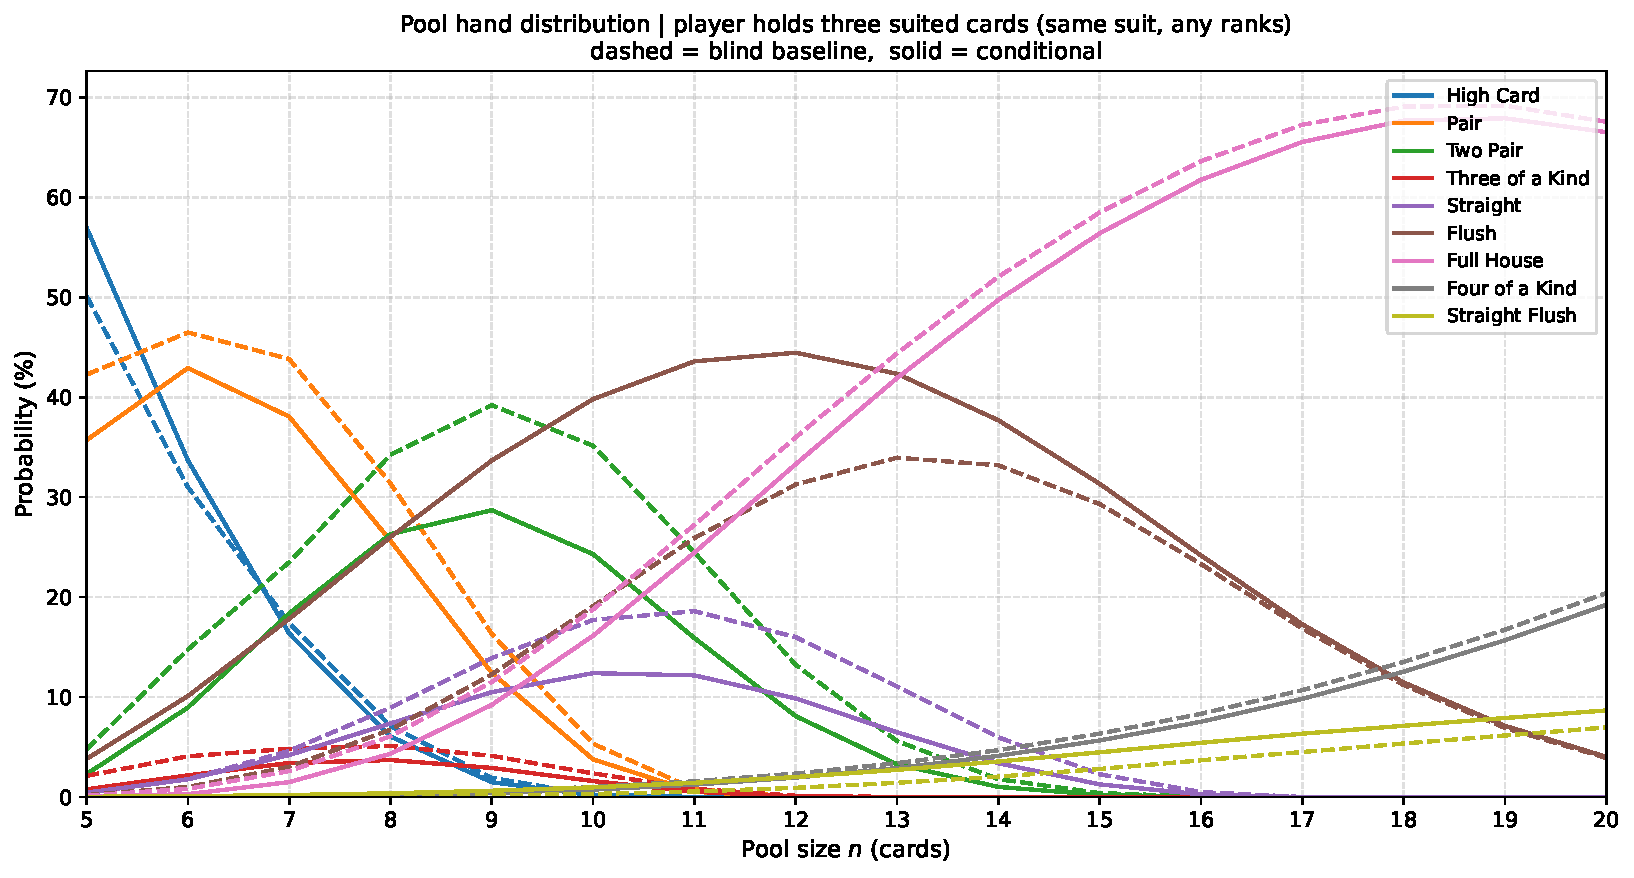
\includegraphics[width=\textwidth]{figures/conditional_3suited.pdf}
    \caption{Conditional pool-hand distribution given the player holds
             \emph{three suited cards} (same suit, any ranks).
             Dashed = blind baseline; solid = conditional.}
    \label{fig:cond_3suited}
\end{figure}

\begin{figure}[h!]
    \centering
    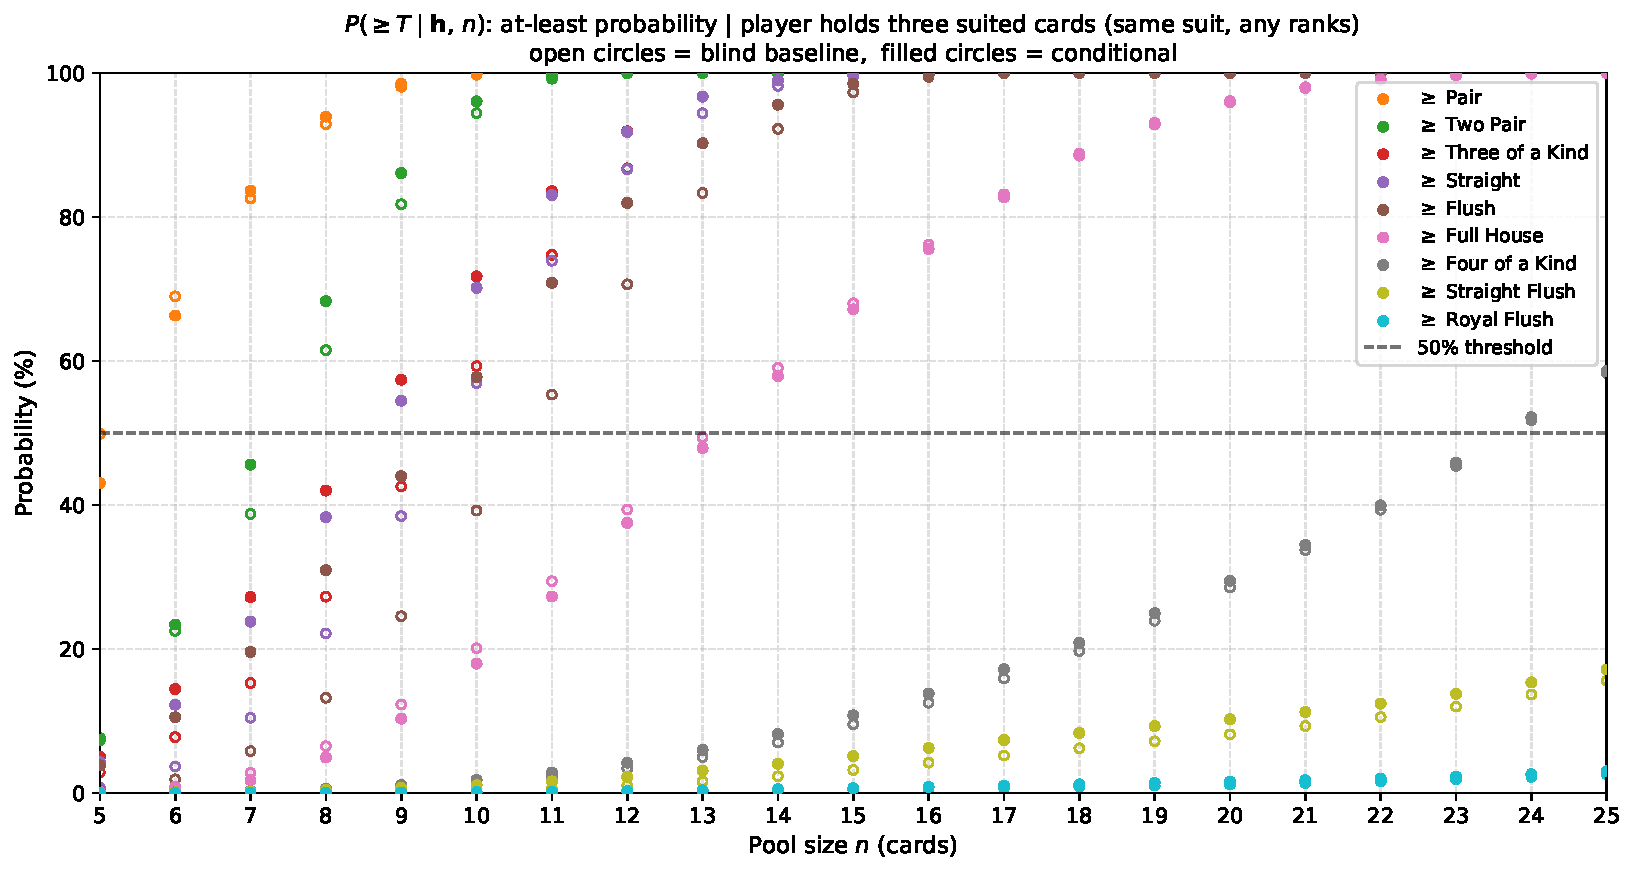
\includegraphics[width=\textwidth]{figures/conditional_3suited_atleast.pdf}
    \caption{Cumulative at-least probability $P(\geq T \mid \mathbf{h}, n)$ given
             the player holds \emph{three suited cards}.
             Open circles = blind baseline; filled circles = conditional; dashed = 50\% threshold.}
    \label{fig:cond_3suited_al}
\end{figure}

Holding two suited cards produces a moderate elevation in Flush probability.
At $n = 7$, the Flush probability rises by $+3.5$ pp to $6.5\%$; at $n = 10$ by $+6.0$ pp to
$25.1\%$.
The effect narrows to $+1.6$ pp at $n = 14$ and is negligible at $n = 20$, reflecting the
diminishing marginal contribution of two suit-matched private cards as the pool grows.

Holding three suited cards produces substantially larger Flush elevation.
At $n = 7$, Flush rises by $+14.8$ pp to $17.8\%$ (approximately $4.2\times$ the baseline rate),
while Pair and Two Pair are each suppressed by roughly $5$--$6$ pp.
At $n = 10$, Flush reaches $39.8\%$ ($+20.7$ pp), making it the single most probable pool
outcome; Straight is reduced by $5.3$ pp and Two Pair by $10.8$ pp.
At $n = 14$, the Flush elevation narrows to $+4.5$ pp ($37.7\%$ vs.\ $33.2\%$), and Straight
Flush rises to $3.6\%$ ($+1.5$ pp).
At $n = 20$, a residual Straight Flush premium of $+1.7$ pp ($8.7\%$ vs.\ $7.0\%$) persists.
These figures support Flush bids at small to moderate pool sizes and Straight Flush bids at
larger pools when holding three suited private cards.

\clearpage
\subsubsection{Adjacent and Range Cards}

\begin{figure}[h!]
    \centering
    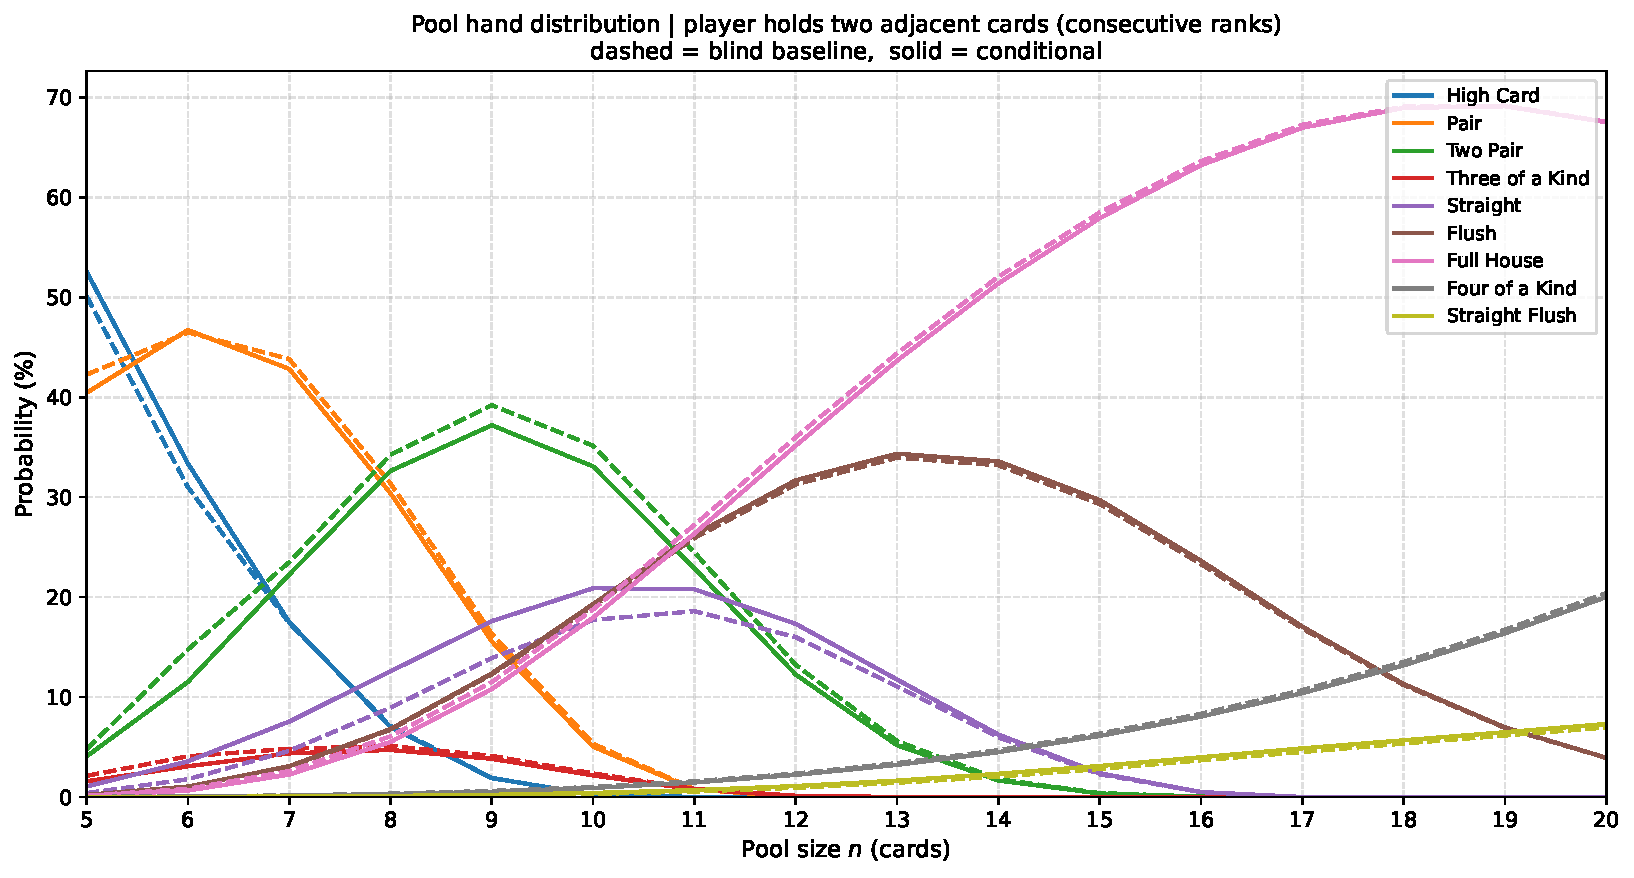
\includegraphics[width=\textwidth]{figures/conditional_adjacent.pdf}
    \caption{Conditional pool-hand distribution given the player holds two
             \emph{adjacent cards} (consecutive ranks, any suits).
             Dashed = blind baseline; solid = conditional.}
    \label{fig:cond_adjacent}
\end{figure}

\begin{figure}[h!]
    \centering
    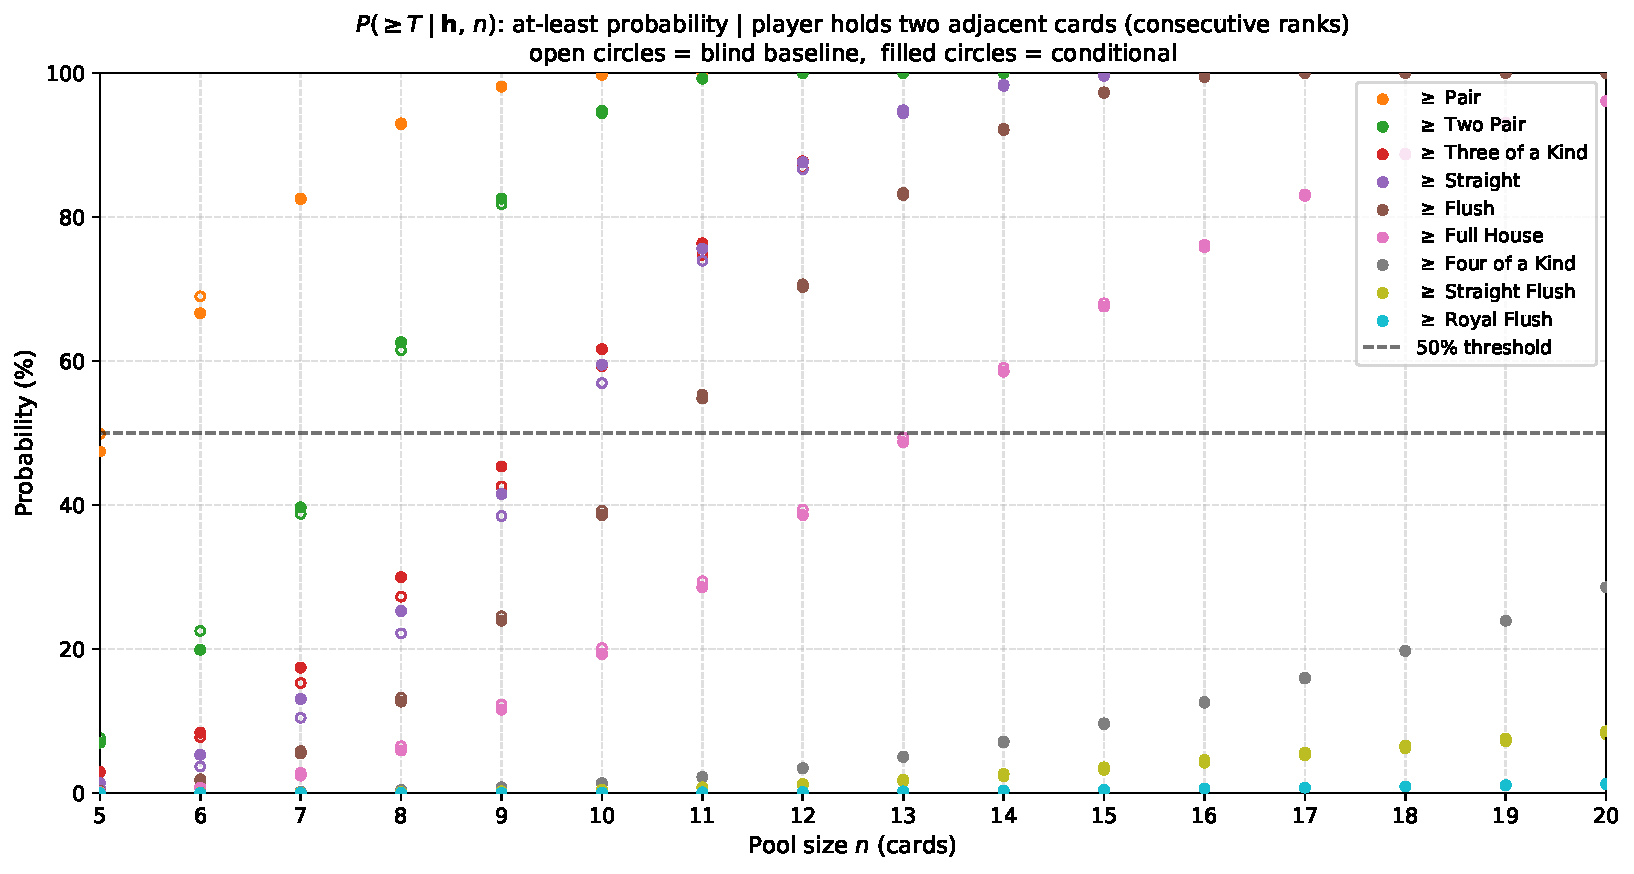
\includegraphics[width=\textwidth]{figures/conditional_adjacent_atleast.pdf}
    \caption{Cumulative at-least probability $P(\geq T \mid \mathbf{h}, n)$ given
             the player holds \emph{two adjacent cards} (consecutive ranks).
             Open circles = blind baseline; filled circles = conditional; dashed = 50\% threshold.}
    \label{fig:cond_adjacent_al}
\end{figure}

\begin{figure}[h!]
    \centering
    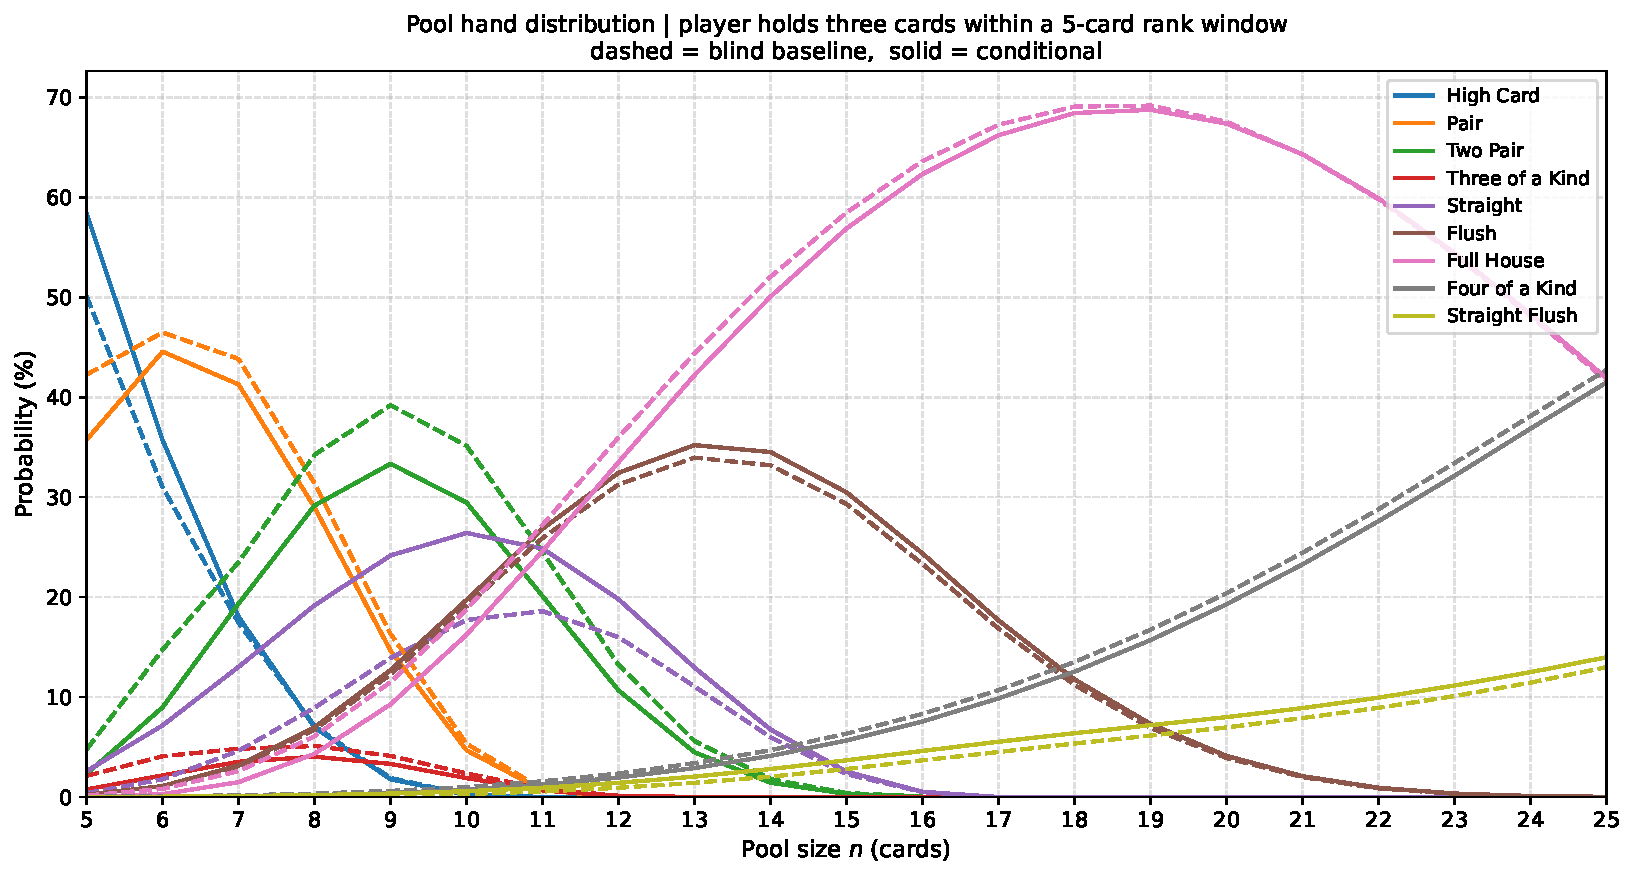
\includegraphics[width=\textwidth]{figures/conditional_3range.pdf}
    \caption{Conditional pool-hand distribution given the player holds
             \emph{three cards within a 5-card rank window}
             (all ranks satisfy $\max - \min \leq 4$).
             Dashed = blind baseline; solid = conditional.}
    \label{fig:cond_3range}
\end{figure}

\begin{figure}[h!]
    \centering
    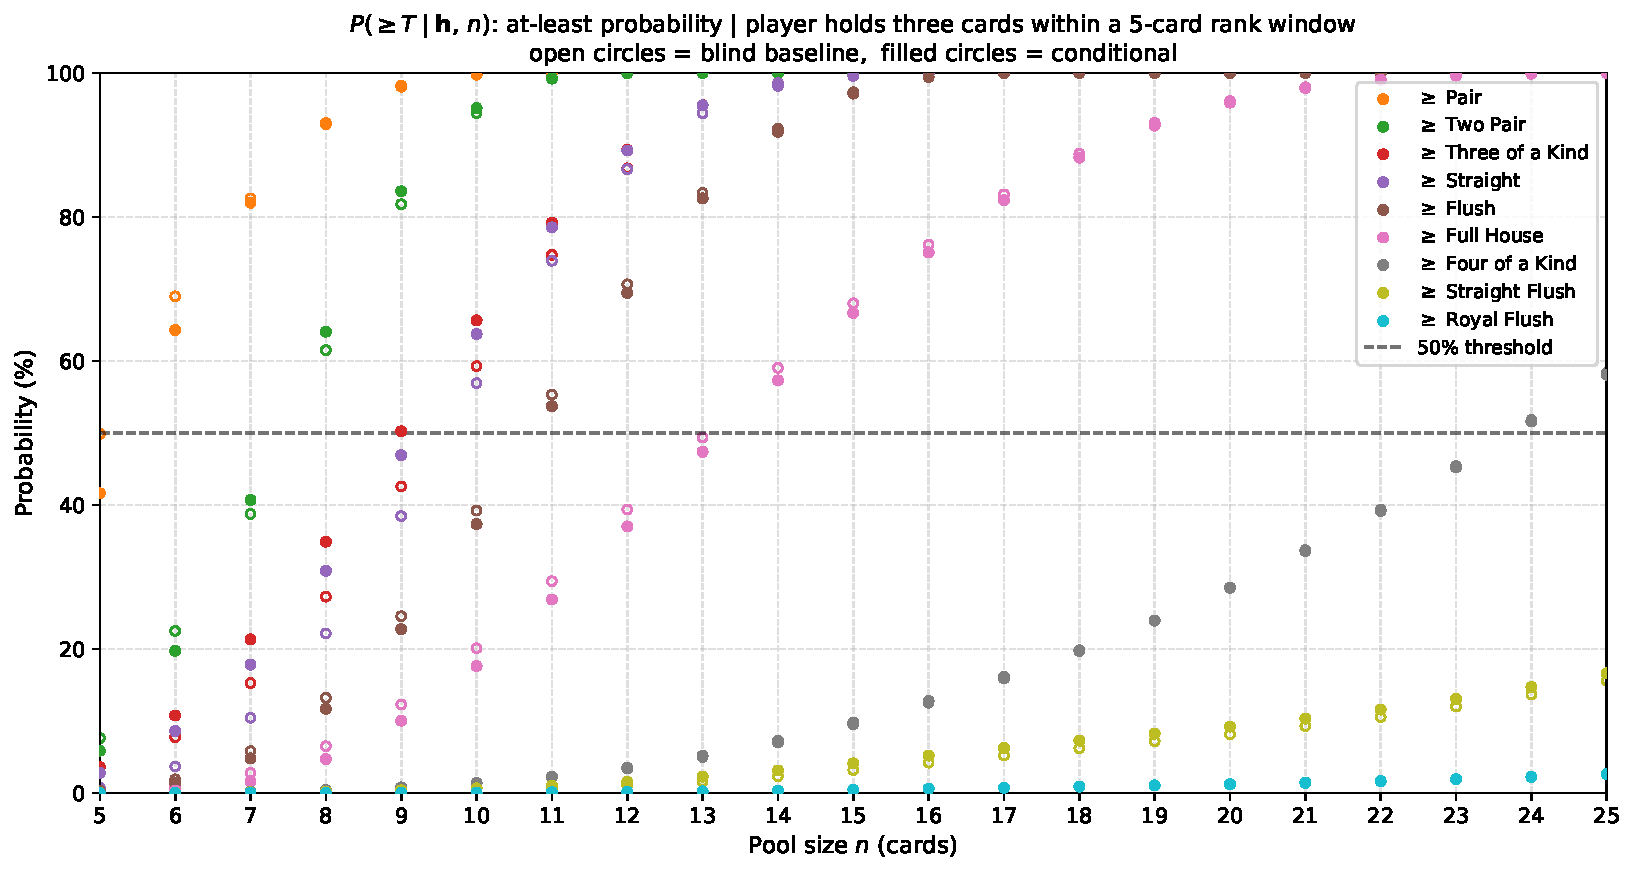
\includegraphics[width=\textwidth]{figures/conditional_3range_atleast.pdf}
    \caption{Cumulative at-least probability $P(\geq T \mid \mathbf{h}, n)$ given
             the player holds \emph{three cards within a 5-card rank window}.
             Open circles = blind baseline; filled circles = conditional; dashed = 50\% threshold.}
    \label{fig:cond_3range_al}
\end{figure}

Holding two adjacent cards produces a modest but consistent Straight elevation.
At $n = 7$, the Straight probability rises by $+2.9$ pp to $7.5\%$; at $n = 10$ by $+3.2$ pp
to $20.9\%$.
No significant deviations from baseline are observed at $n \geq 14$, indicating that the
informational advantage of two consecutive private ranks is absorbed by the larger pool.

Holding three cards within a 5-card rank window produces substantially larger Straight elevation.
At $n = 7$, Straight rises by $+8.4$ pp to $13.0\%$ (approximately $2.8\times$ the baseline
rate), while Two Pair is suppressed by $4.1$ pp and Three of a Kind by $1.3$ pp.
At $n = 10$, the Straight elevation reaches $+8.7$ pp ($26.4\%$ vs.\ $17.7\%$), with Two Pair
suppressed by $5.7$ pp.
The effect narrows sharply at $n = 14$ (Full House $-2.0$ pp; Flush $+1.3$ pp) and is
negligible by $n = 20$, where only a $+1.0$ pp residual Straight Flush elevation persists.

\clearpage
\subsubsection{Information Value of Private Cards}

The analyses in the preceding subsubsections directly quantify the strategic value of private
hand knowledge across six conditions.
The paired and grouped conditions produce the largest rank-based deviations: a pair
systematically elevates Full House and suppresses Flush and Straight, while trips eliminates
lower hand categories entirely and drives Full House to $70\%$ or greater at moderate pool sizes.
The suited conditions produce the most pronounced Flush elevation, with three suited cards
raising the Flush probability to nearly $40\%$ at $n = 10$, a shift large enough to change
the optimal bid type relative to blind strategy.
The adjacent conditions produce the weakest deviations overall, with two adjacent cards providing
only a $3$ pp Straight premium that diminishes above $n = 14$.
A formal treatment of information value via Kullback--Leibler divergence across all
private-hand configurations is planned for subsequent work.

\clearpage
\subsubsection{Rank-Level Bid Thresholds}
\label{sec:thresholds}

The preceding analysis identifies which \emph{hand type} straddles the 50\% cumulative
probability threshold for each condition and pool size.  In practice, bids are made at the
level of both hand type \emph{and} primary rank: bidding ``Pair'' without specifying a rank is
not a valid move.  A more precise question is therefore: given pool size $n$ and private-hand
condition, what is the strongest bid $(T, r)$ such that
\[
    P\!\left(\mathrm{BestHand} \geq (T,r) \;\middle|\; \mathbf{h},\, n\right) \;\geq\; 0.50\,?
\]
We call this the \emph{threshold bid}.  Everything at or below the threshold bid is a
``positive-expectation'' bid (more likely true than false); everything above it is a
``negative-expectation'' bid.

For each condition and pool size we locate the pair $(T_{\mathrm{above}}, r_{\mathrm{above}})$
and $(T_{\mathrm{below}}, r_{\mathrm{below}})$ whose cumulative at-least probabilities bracket
50\%, using the bid ordering of Definition~2: bids are ordered first by hand type, then by
primary rank within a type.  The primary rank encodes: the pair rank for Pair; the higher pair
rank for Two Pair; the trip rank for Three of a Kind, Full House; the quad rank for Four of a
Kind; the straight high card for Straight and Straight Flush; the flush high card for Flush; and
always Ace for Royal Flush.

Tables~\ref{tab:threshold_part1} and \ref{tab:threshold_part2} display these threshold bids for
all seven scenarios (blind and six conditional conditions) across pool sizes $n = 5$ to $25$.
Each cell shows the bid label (e.g.\ \textbf{FH A} for Full House with trip rank Ace), its
cumulative probability, and a canonical $n$-card example pool.  Both tables are generated by
\texttt{compute\_conditional\_probs.py} from $10^6$ Monte Carlo samples per condition
($3 \times 10^6$ for the blind scenario).

\begin{figure}[htbp]
    \centering
    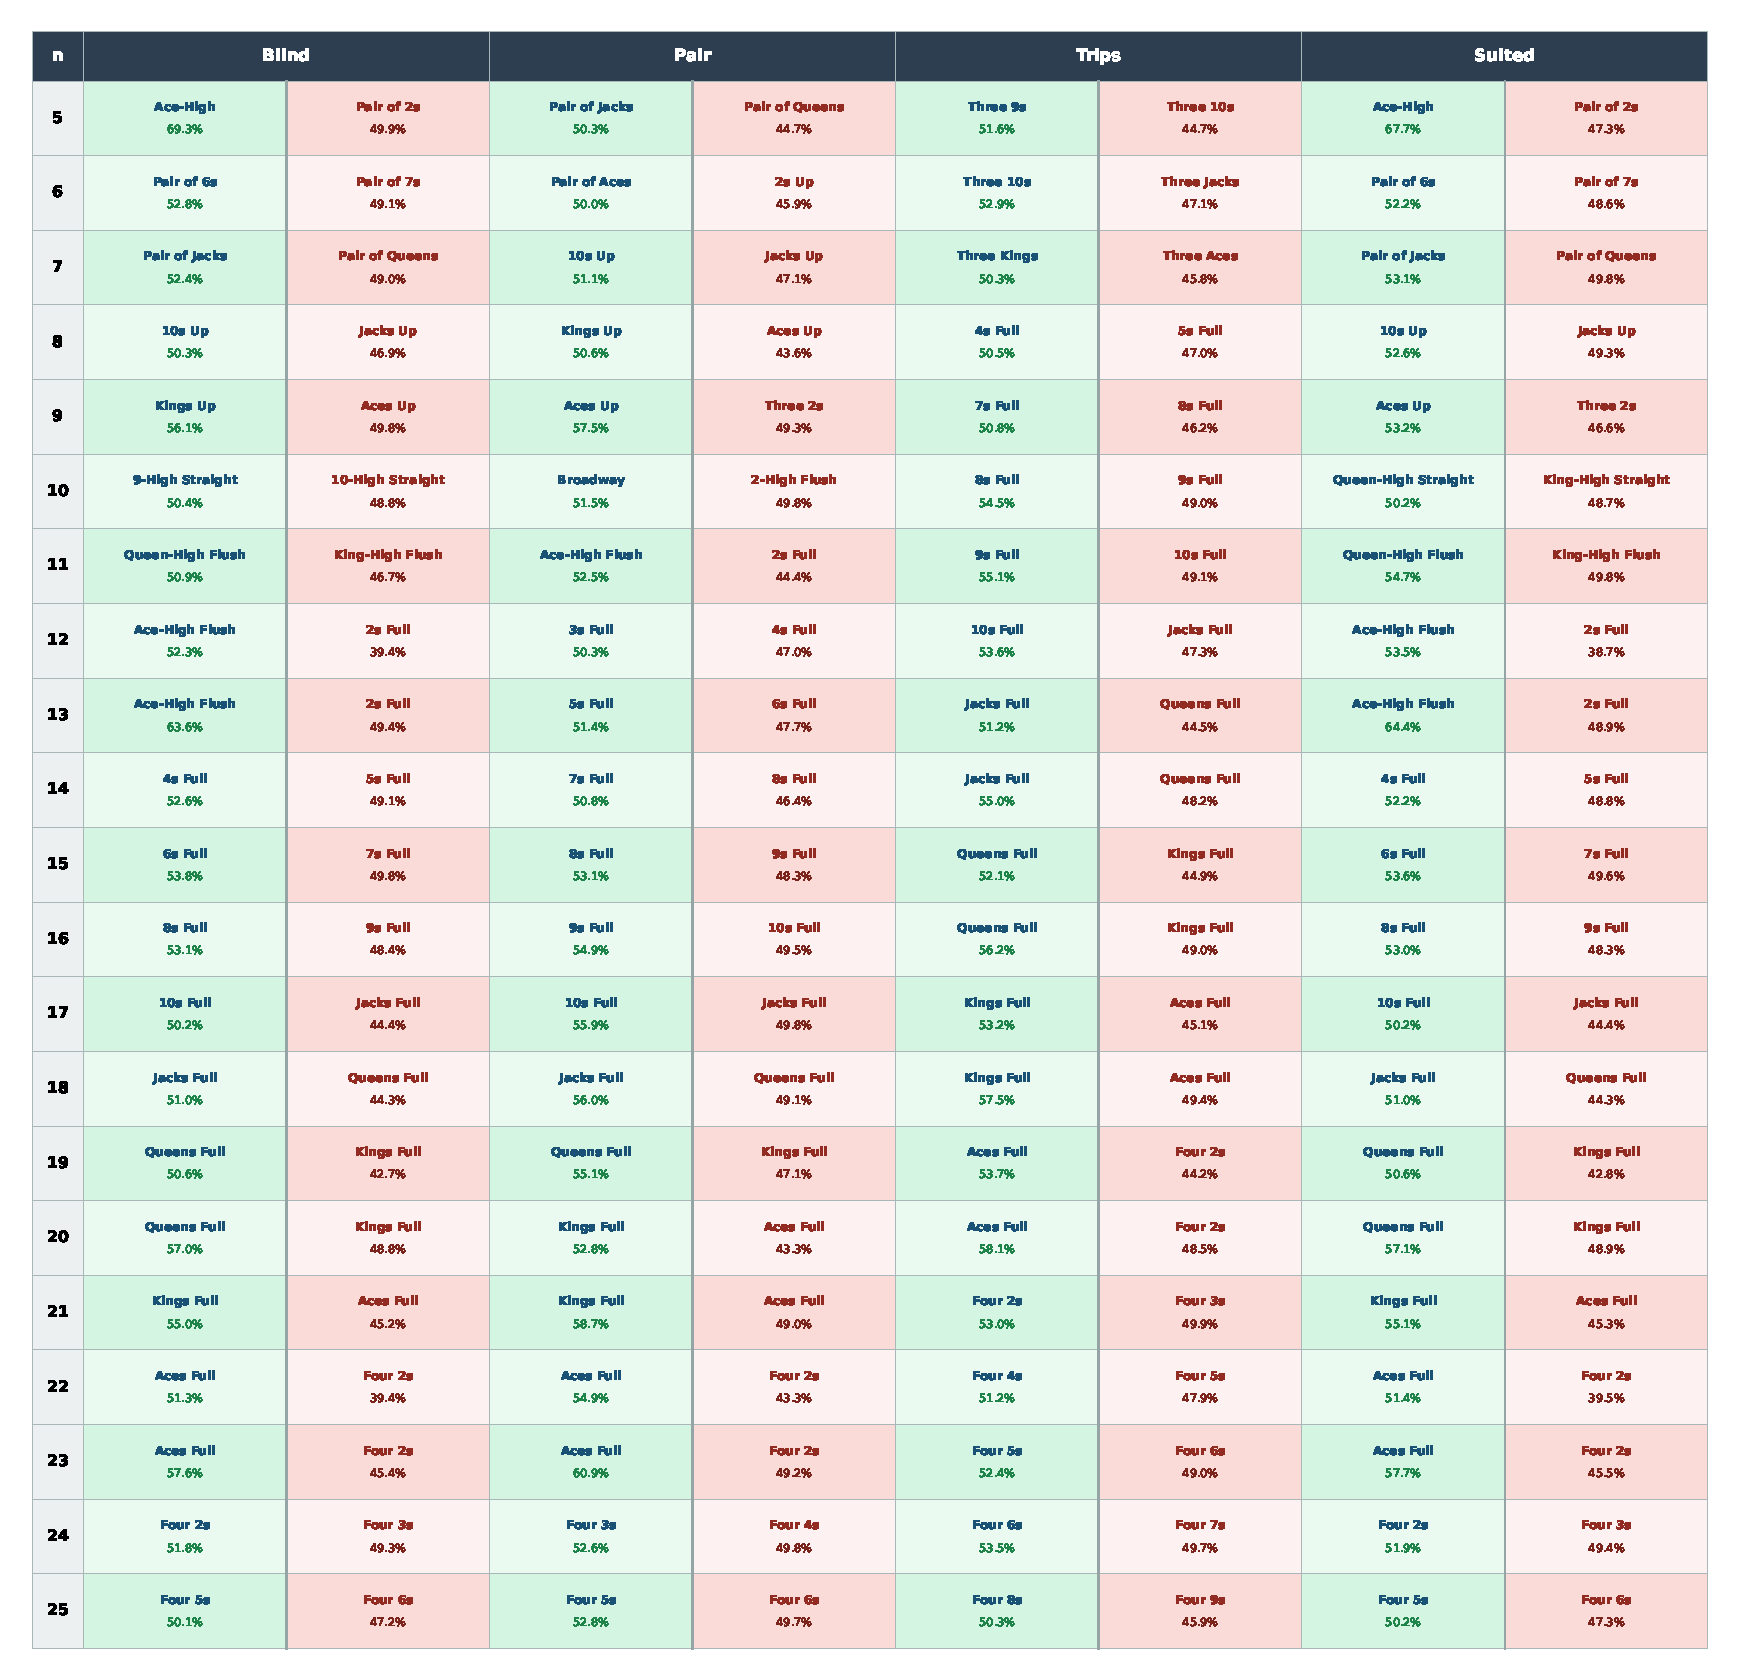
\includegraphics[width=\textwidth]{figures/tables/threshold_part1.pdf}
    \caption{Rank-level bid thresholds for the blind scenario and three private-hand
             conditions (Pair, Trips, Suited). Each cell is split left/right:
             the green left half shows the strongest bid $(T,r)$ with
             $P(\geq(T,r))\geq 50\%$, and the red right half shows the next
             stronger bid whose probability falls just below 50\%.
             Generated by \texttt{compute\_conditional\_probs.py}.}
    \label{fig:threshold_part1}
\end{figure}

\begin{figure}[htbp]
    \centering
    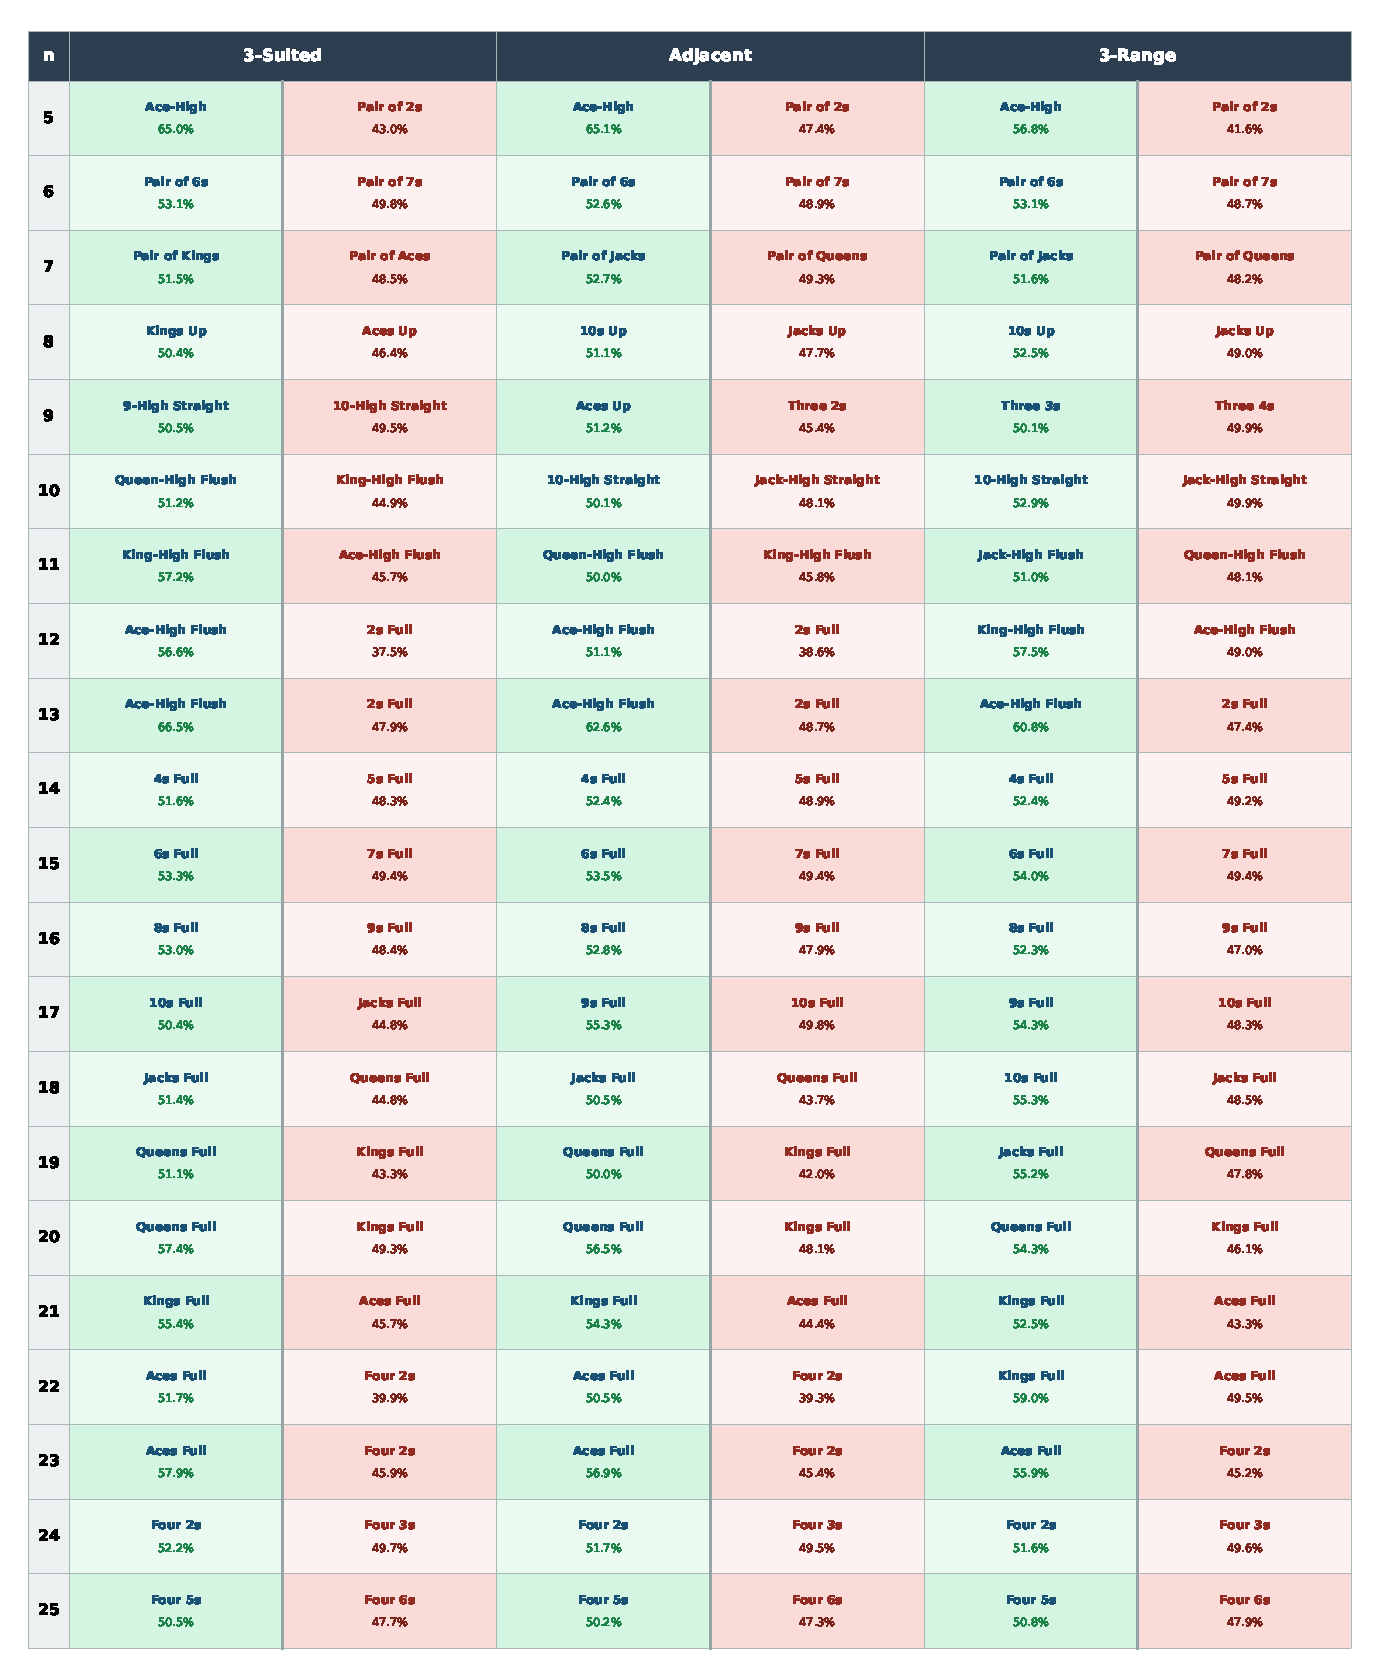
\includegraphics[width=\textwidth]{figures/tables/threshold_part2.pdf}
    \caption{Rank-level bid thresholds for three additional private-hand conditions
             (3-Suited, Adjacent, 3-Range). Cell format as in Figure~\ref{fig:threshold_part1}.}
    \label{fig:threshold_part2}
\end{figure}

\section{Future Work: Nash Equilibrium via Regularized Nash Dynamics}
\label{sec:future}

The combinatorial analysis of Sections~\ref{sec:blind} and \ref{sec:conditional}
provides the information-theoretic foundation for strategic play. The next phase of
this project is to approximate the Nash equilibrium of the game using Regularized Nash
Dynamics (RND), a policy-gradient framework for imperfect-information games introduced
in the context of Liar's Poker by~\cite{rnd_paper}.

\subsection{Game-Theoretic Framework}

We model the game as an extensive-form game with imperfect information. The information
state of each player consists of:
\begin{itemize}
    \item their own cards (observed),
    \item the sequence of bids made so far (public),
    \item the number of cards held by each player (public).
\end{itemize}
The action space at each information set is the set of valid bids (strictly higher
than the current bid) plus the call action. The game is zero-sum in the sense that
exactly one player wins.

\subsection{Regularized Nash Dynamics}

RND stabilizes the self-play training loop by adding an entropy regularization term
that anchors the current policy toward a periodically updated reference policy. The
update rule at training step $t$ is:
\[
\pi_{t+1} = \arg\max_{\pi} \;\mathbb{E}_{\pi}[G] - \eta \cdot \mathrm{KL}(\pi \,\|\, \bar{\pi}_t),
\]
where $G$ is the game value, $\eta$ is a regularization coefficient, and $\bar{\pi}_t$
is the reference policy. The reference is updated every fixed number of steps to
encourage exploration. The OpenSpiel framework~\cite{openspiel} provides a principled
computational environment for implementing and evaluating this training loop.

\subsection{Implementation Plan}

The implementation will proceed in three stages:
\begin{enumerate}
    \item \textbf{Two-player, fixed pool size.} Solve the two-player game with fixed
          hand sizes (no card accumulation) to establish a baseline equilibrium.
    \item \textbf{Two-player, full dynamics.} Add the card accumulation and
          elimination mechanic to study how the equilibrium shifts near the
          elimination boundary ($h_i = 4$).
    \item \textbf{Multiplayer extension.} Generalize to $k \in \{3, 4, 5\}$ players,
          where coalition-like dynamics may emerge even in a nominally zero-sum setting.
\end{enumerate}
The probability tables from Section~\ref{sec:prob} serve as oracle lookup tables
within the agent's value network, reducing the computational burden of on-the-fly
probability estimation during self-play.

\section{Conclusion}

This paper establishes the combinatorial foundations for rational play in card-based
Liar's Poker. Exact and high-precision Monte Carlo probability tables for pool sizes
$n = 5$ through $n = 25$ enable principled blind bidding strategies, and conditional
probability analysis quantifies the strategic value of private card information. These
results will directly inform the design of a Regularized Nash Dynamics agent in
subsequent work, which aims to approximate the true Nash equilibrium of the game and
provide strategic insights unavailable from purely combinatorial analysis.

\printbibliography

\end{document}
